%%%%%%%%%%%%%%%%%%%%%%%%%%%%%%%%%%%%%%%%%%%%%%%%%%%%%%%%%%%%%%%%%%%%%%%%%%%%%%%%
%%
%% Para utilizar ese modelo sao necessarios os seguintes arquivos:
%%
%% copin.cls
%% copin.sty
%% mestre.sty
%%
%%%%%%%%%%%%%%%%%%%%%%%%%%%%%%%%%%%%%%%%%%%%%%%%%%%%%%%%%%%%%%%%%%%%%%%%%%%%%%%%

\documentclass[a4paper,titlepage]{copin}
\usepackage[portuges,english]{babel}
\usepackage{copin,mestre,epsfig}
\usepackage{times}

%-------------------------- Para usar acentuacaoo em sistemas ISO8859-1 ------------------------------------
% Se estiver usando o Microsoft Windows ou linux com essa codificacao, descomente essa linhas abaixo
% e comente as linhas referentes ao UTF8
%\usepackage[latin1]{inputenc} % Usar acentuacao em sistemas ISO8859-1, comentar a linha com  \usepackage[utf8x]{inputenc}
%-----------------------------------------------------------------------------------------------------

%-------------------------- Para usar acentuacao em sistemas UTF8 ------------------------------------
% Para a maior parte das distribuicoes linux, usar a opcao utf8x (lembrar de comentar as linha referente a ISO8859-1 acima)
\usepackage{ucs}
%\usepackage[utf8x]{inputenc}
\usepackage[utf8]{inputenc}
\usepackage[T1]{fontenc}
%-----------------------------------------------------------------------------------------------------


\usepackage{fancyheadings}
\usepackage{graphicx}
\usepackage{longtable} %tabelas longas, para tabelas que ultrapassam uma pagina
%\input{psfig.sty}

% ----------------- Para inserir gráficos no formato .eps -----------------
\usepackage{epstopdf}

% ----------------- Para inserir URLs -----------------
\usepackage{url}

% ----------------- Para inserir texto colorido -----------------
\usepackage{color}

% ----------------- Para inserir o índice no pdf gerado -----------------
\usepackage{hyperref}
\hypersetup{colorlinks=true,allcolors=black}
\usepackage{hypcap}

% ----------------- Para colocar imagens e tabelas dentro das seções -----------------
\usepackage{float}

% ----------------- Para inserir equações -----------------
\usepackage{amsmath}

\usepackage{multirow}

% ----------------- Para inserir codigo fonte de linguagens de programacao no documento -------------
\usepackage{listings}
\lstset{numbers=left,
stepnumber=1,
firstnumber=1,
%numberstyle=\tiny,
extendedchars=true,
breaklines=true,
frame=tb,
basicstyle=\footnotesize,
stringstyle=\ttfamily,
showstringspaces=false
}
\renewcommand{\lstlistingname}{Código Fonte}
\renewcommand{\lstlistlistingname}{Lista de Códigos Fonte}
% ---------------------------------------------------------------------------------------------------

\selectlanguage{portuges}
\sloppy



\begin{document}



%%%%%%%%%%%%%%%%%%%%%%%%%%%%%%%%%%%%%%%%%%%%%%%%%%%%%%%%%%%%%%%%%%%%%%%%%%%%%%%%
\Titulo{Título da Dissertação}
\Autor{Arthur Silva Freire}
\Data{dd/mm/aaaa}
\Area{Ciência da Computação}
\Pesquisa{Engenharia de \textit{Software}}
\Orientadores{Hyggo Oliveira de Almeida  \\
              Angelo Perkusich  \\
	         (Orientadores)}

\newpage
\cleardoublepage

\PaginadeRosto

\newpage
\cleardoublepage

%%%%%%%%%%%%%%%%%%%%%%%%%%%%%%%%%%%%%%%%%%%%%%%%%%%%%%%%%%%%%%%%%%%%%%%%%%%%%%%%
\begin{resumo}
Resumo aqui

\end{resumo}

\newpage
\cleardoublepage

%%%%%%%%%%%%%%%%%%%%%%%%%%%%%%%%%%%%%%%%%%%%%%%%%%%%%%%%%%%%%%%%%%%%%%%%%%%%%%%%
\begin{summary}
Abstract Here




\end{summary}

\newpage
\cleardoublepage

%%%%%%%%%%%%%%%%%%%%%%%%%%%%%%%%%%%%%%%%%%%%%%%%%%%%%%%%%%%%%%%%%%%%%%%%%%%%%%%%
\begin{agradecimentos}
Agradecimentos aqui
\end{agradecimentos}

\clearpage

%%%%%%%%%%%%%%%%%%%%%%%%%%%%%%%%%%%%%%%%%%%%%%%%%%%%%%%%%%%%%%%%%%%%%%%%%%%%%%%%
%% Definicao do cabecalho: secao do lado esquerdo e numero da pagina do lado direito
\pagestyle{fancy}
\addtolength{\headwidth}{\marginparsep}\addtolength{\headwidth}{\marginparwidth}\headwidth = \textwidth
\renewcommand{\chaptermark}[1]{\markboth{#1}{}}
\renewcommand{\sectionmark}[1]{\markright{\thesection\ #1}}\lhead[\fancyplain{}{\bfseries\thepage}]%
	     {\fancyplain{}{\emph{\rightmark}}}\rhead[\fancyplain{}{\bfseries\leftmark}]%
             {\fancyplain{}{\bfseries\thepage}}\cfoot{}

%%%%%%%%%%%%%%%%%%%%%%%%%%%%%%%%%%%%%%%%%%%%%%%%%%%%%%%%%%%%%%%%%%%%%%%%%%%%%%%%
\selectlanguage{portuges}

\Sumario
\ListadeSimbolos
\listoffigures
\listoftables
%\lstlistoflistings %lista de codigos fonte - Para inserir a listagem de codigos fonte
\newpage
\cleardoublepage

\Introducao


%%%%%%%%%%%%%%%%%%%%%%%%%%%%%%%%%%%%%%%%%%%%%%%%%%%%%%%%%%%%%%%%%%%%%%%%%%%%%%%%
%
% Hifenizacao - Colocar lista de palavras que nao devem ser separadas e que
% nao estao no dicionario portugues.
% As palavras do dicionario portugues ja sao separadas corretamente pelo lateX
%
\hyphenation{ Hardware Software etc  }


%%%%%%%%%%%%%%%%%%%%%%%%%%%%%%%%%%%%%%%%%%%%%%%%%%%%%%%%%%%%%%%%%%%%%%%%%%%%%%%%
%% A partir daqui coloque seus capitulos. Sugere-se que eles sejam inseridos com o comando \input
%% Da seguinte maneira:
%%
%% \chapter{Introdução}
\label{intro}

De acordo com Emam et al. \cite{emam}, a porcentagem de projetos de TI que sucedem varia entre 46 e 55 porcento. De acordo com os autores, o sucesso de projetos de TI depende de cinco fatores: satisfação do cliente, orçamento, cronograma, qualidade do produto e produtividade da equipe. Além disso, para uma disciplina aplicada, esses números representam um alto índice de falhas.

Boehm et al. \cite{boehm} identificaram seis principais razões de falha em projetos de \textit{software}: requisitos imcompletos, ausência de envolvimento do cliente, falta de recursos, expectativas irrealistas, ausência de suporte executivo e mudança de requisitos e especificações. A ocorrência da maioria desses fatores se dá por conta de problemas na comunicação e interação entre desenvolvedores e \textit{stakeholders}. Uma das principais razões pelas quais as metodologias ágeis têm se tornado popular no contexto do desenvolvimento de \textit{software}, é a necessidade de focar na melhoria da colaboração entre desenvolvedores e \textit{stakeholders}, além de melhorar a velocidade de resposta com relação à mudança de requisitos.

No Manifesto Ágil \cite{manifesto}, há afirmações que projetos que utilizam métodos ágeis devem focar nos indivíduos e nas relações entre eles em vez de focar em processos e ferramentas. Além disso, como é esperado que as equipes ágeis sejam auto-organizáveis, é necessário que os membros da equipe colaborem entre si e adotem os conceitos de responsabilidade e compromisso com as atividades da equipe. De acordo com Bustamante et al. \cite{bustamante}, numa equipe ágil ideal, os membros da equipe compartilham o mesmo ambiente de trabalho e comunicam-se cara-a-cara diariamente. Lalsing et al. \cite{lalsing} afirmam que o gerente de projeto deve definir as relações entre os papéis para garantir a efetividade na coordenação da equipe e o controle do projeto. Nesse último trabalho, os autores também afirmam que indivíduos com diferentes personalidades, geralmente, devem trabalhar juntos para garantir uma equipe coesa.

A utilização de metodologias ágeis requer a adoção de uma série de práticas que aumentam as chances de sucesso do projeto, pois a adoção dessas práticas resolve a maioria dos problemas responsáveis por falhas em projetos de \textit{software}. Assim, uma vez que a saída de um processo de \textit{software} é o próprio \textit{software}, a qualidade do produto final é dependente de uma série de artefatos e fatores que compõem esse processo.

Chow et al. \cite{chow}, identificaram os três principais fatores que influenciam o sucesso de projetos de desenvolvimento de \textit{software} que utilizam métodos ágeis: estratégia de entrega, técnicas de engenharia de \textit{software} no contexto ágil e a capacidade do time. Esse último, de acordo com os autores, está relacionado com o ato de construir projetos em volta de indivíduos motivados. Tendo em vista que as equipes são consideradas os recursos mais valiosos de projetos que utilizam métodologias ágeis, e sua capacidade, como citado anteriormente, é um dos principais fatores que influenciam o sucesso desses projetos, faz-se necessário atentar para os aspectos que influenciam a eficiência dessas equipes.

Em algumas pesquisas sobre equipes de desenvolvimento de \textit{software}, foi identificado que a eficiência dessas equipes está relacionada a eficiência da coordenação do trabalho em equipe \cite{kraut} \cite{hoegl}. Logo, se a eficiência do trabalho em equipe está relacionada com a eficiência das equipes, que por sua vez, influenciam o sucesso de projetos de desenvolvimento de \textit{software}, pode-se afirmar que a eficiência do trabalho em equipe também está relacionada com o sucesso desses projetos. Assim, a avaliação e melhora contínua da eficiência do trabalho em equipe é importante para garantir boa qualidade do \textit{software} resultante de um processo, assim como o sucesso do projeto.

\section{Problemática}
\label{intro:prob}

Conforme supracitado, é importante avaliar e garantir a melhoria contínua da ETE, a adoção de um método que proporcione essas oportunidades aos gerentes de projeto agregará valor à esses projetos. Contudo, há diversos fatores que podem vir a influenciar essa eficiência \cite{}. Apesar do contexto em que o objeto de estudo foi avaliado neste trabalho ser restrito, algumas equipes podem decidir utilizar determinadas práticas que outras equipes não utilizam. Esse fato pode causar diferença entre os conjuntos de fatores que influenciam a ETE de diferentes equipes.

Além disso, os fatores que influenciam a ETE, são, em sua grande maioria, subjetivos. Dessa forma, a aplicação de um método de avaliação da ETE precisa minimizar o viés que pode ser introduzido por conta da subjetividade desses fatores, garantindo que os resultados sejam fiéis ao cenário no qual a avaliação foi realizada.

\section{Objetivos}
\label{intro:obj}

Considerando o que foi abordado na seções anteriores, o principal objetivo deste trabalho é mitigar os problemas descritos, principalmente na Seção \ref{intro:prob}, propondo uma abordagem para auxiliar os gerentes de projeto na avaliação da ETE de equipes baseadas em \textit{Scrum}. Além disso, a utilização dessa abordagem deve auxiliar na identificação de oportunidades de melhorias no trabalho em equipe.

Como forma de representar a ETE em função do relacionamento dos fatores que a influenciam, optou-se pelo uso de \textit{Redes Bayesianas}, uma vez que modelos probabilísticos dessa família são adequados para se modelar incerteza em um determinado domínio \cite{bengal}. Essa decisão foi tomada com o objetivo de diminuir a incerteza em relação à confiança nos resultados finais do modelo, tendo em vista que, como citado na Seção \ref{intro:prob}, a maioria dos fatores que influenciam a ETE são subjetivos.

\subsection{Objetivos Específicos}
\label{intro:obj:esp}

Para simplificar os objetivos descritos na Seção \ref{intro:obj}, podemos especificá-los da seguinte maneira:

\begin{enumerate}
  \item Propor uma abordagem baseada em \textit{Redes Bayesianas} para auxiliar na avaliação da ETE de equipes baseadas em \textit{Scrum};
  \item Proporcionar aos gerentes de projeto uma abordagem menos sensível à subjetividade na avaliação da ETE, que possa auxiliar na identificação de oportunidades de melhorias no trabalho em equipe;
  \item Aplicar a abordagem em projetos reais de desenvolvimento de \textit{software}, baseados em \textit{Scrum}, para avaliar sua utilidade e seu custo-benefício.
\end{enumerate}

\section{Contribuições e Resultados}
\label{intro:result}

A abordagem proposta neste trabalho é dividida em etapas que englobam desde a concepção do modelo baseado em \textit{Redes Bayesianas} até a avaliação dos resultados calculados por ele. A utilização de modelos dessa família permite calcular probabilisticamente o impacto de fatores menos complexos (nós de entrada e nós intermediários) que afetam a ETE. Tendo em mãos esses resultados, os gerentes poderão observar as saídas do modelo, que o auxiliarão na identificação de oportunidades de melhorias no trabalho em equipe.

Mesmo sabendo que o conjuntos de fatores que influenciam a ETE de determinadas equipes podem ser diferentes, neste trabalho é proposto um modelo genérico para representar a ETE no contexto de \textit{Scrum}. Dessa forma, os indivíduos que desejarem utilizar essa abordagem poderão adotá-lo como base para modificá-lo e, assim, obtenham uma representação mais fiel em relação ao cenário em que a equipe está inserida.

{\color{red} Os resultados serão inseridos ao final do estudo de caso...}

\section{Relevância}
\label{intro:rel}

A abordagem proposta é uma alternativa promissora para auxiliar no processo de tomada de decisões por parte dos gerentes de projeto. Os resultados calculados pelo modelo permitem que eles avaliem quais fatores merecem mais atenção caso mais de um fator esteja dimnuindo a ETE, e quais atitudes podem ser tomadas para evitar riscos, além de quais atitudes podem ser tomadas para melhorar a EFT. Essas oportunidades de auxílio na tomada de decisões por parte dos gerentes existem porque, com a utilização dessa abordagem, é possível interpretar fatores subjetivos de forma mais objetiva.

Como a abordagem proposta proporciona os benefícios supracitados, e sabendo da relação entre a EFT e a qualidade do produto de \textit{software} resultante do processo, e também o processo em si, a sua utilização proporciona um aumento nas chances de sucesso do projeto. Além disso, essa abordagem pode ser integrada com outras abordagens que utilizadas na avaliação do processo de \textit{software} como um todo.

\section{Estrutura da Dissertação}
\label{intro:estr}

Esta dissertação está organizada da seguinte forma:

...

%% \chapter{Fudamentação Teórica}
\label{fund}

\chapter{Introdução}
\label{intro}

De acordo com Emam et al. \cite{emam}, a porcentagem de projetos de TI que sucedem varia entre 46 e 55 porcento. De acordo com os autores, o sucesso de projetos de TI depende de cinco fatores: satisfação do cliente, orçamento, cronograma, qualidade do produto e produtividade da equipe. Além disso, para uma disciplina aplicada, esses números representam um alto índice de falhas.

Boehm et al. \cite{boehm} identificaram seis principais razões de falha em projetos de \textit{software}: requisitos imcompletos, ausência de envolvimento do cliente, falta de recursos, expectativas irrealistas, ausência de suporte executivo e mudança de requisitos e especificações. A ocorrência da maioria desses fatores se dá por conta de problemas na comunicação e interação entre desenvolvedores e \textit{stakeholders}. Uma das principais razões pelas quais as metodologias ágeis têm se tornado popular no contexto do desenvolvimento de \textit{software}, é a necessidade de focar na melhoria da colaboração entre desenvolvedores e \textit{stakeholders}, além de melhorar a velocidade de resposta com relação à mudança de requisitos.

No Manifesto Ágil \cite{manifesto}, há afirmações que projetos que utilizam métodos ágeis devem focar nos indivíduos e nas relações entre eles em vez de focar em processos e ferramentas. Além disso, como é esperado que as equipes ágeis sejam auto-organizáveis, é necessário que os membros da equipe colaborem entre si e adotem os conceitos de responsabilidade e compromisso com as atividades da equipe. De acordo com Bustamante et al. \cite{bustamante}, numa equipe ágil ideal, os membros da equipe compartilham o mesmo ambiente de trabalho e comunicam-se cara-a-cara diariamente. Lalsing et al. \cite{lalsing} afirmam que o gerente de projeto deve definir as relações entre os papéis para garantir a efetividade na coordenação da equipe e o controle do projeto. Nesse último trabalho, os autores também afirmam que indivíduos com diferentes personalidades, geralmente, devem trabalhar juntos para garantir uma equipe coesa.

A utilização de metodologias ágeis requer a adoção de uma série de práticas que aumentam as chances de sucesso do projeto, pois a adoção dessas práticas resolve a maioria dos problemas responsáveis por falhas em projetos de \textit{software}. Assim, uma vez que a saída de um processo de \textit{software} é o próprio \textit{software}, a qualidade do produto final é dependente de uma série de artefatos e fatores que compõem esse processo.

Chow et al. \cite{chow}, identificaram os três principais fatores que influenciam o sucesso de projetos de desenvolvimento de \textit{software} que utilizam métodos ágeis: estratégia de entrega, técnicas de engenharia de \textit{software} no contexto ágil e a capacidade do time. Esse último, de acordo com os autores, está relacionado com o ato de construir projetos em volta de indivíduos motivados. Tendo em vista que as equipes são consideradas os recursos mais valiosos de projetos que utilizam métodologias ágeis, e sua capacidade, como citado anteriormente, é um dos principais fatores que influenciam o sucesso desses projetos, faz-se necessário atentar para os aspectos que influenciam a eficiência dessas equipes.

Em algumas pesquisas sobre equipes de desenvolvimento de \textit{software}, foi identificado que a eficiência dessas equipes está relacionada a eficiência da coordenação do trabalho em equipe \cite{kraut} \cite{hoegl}. Logo, se a eficiência do trabalho em equipe está relacionada com a eficiência das equipes, que por sua vez, influenciam o sucesso de projetos de desenvolvimento de \textit{software}, pode-se afirmar que a eficiência do trabalho em equipe também está relacionada com o sucesso desses projetos. Assim, a avaliação e melhora contínua da eficiência do trabalho em equipe é importante para garantir boa qualidade do \textit{software} resultante de um processo, assim como o sucesso do projeto.

\section{Problemática}
\label{intro:prob}

Conforme supracitado, é importante avaliar e garantir a melhoria contínua da ETE, a adoção de um método que proporcione essas oportunidades aos gerentes de projeto agregará valor à esses projetos. Contudo, há diversos fatores que podem vir a influenciar essa eficiência \cite{}. Apesar do contexto em que o objeto de estudo foi avaliado neste trabalho ser restrito, algumas equipes podem decidir utilizar determinadas práticas que outras equipes não utilizam. Esse fato pode causar diferença entre os conjuntos de fatores que influenciam a ETE de diferentes equipes.

Além disso, os fatores que influenciam a ETE, são, em sua grande maioria, subjetivos. Dessa forma, a aplicação de um método de avaliação da ETE precisa minimizar o viés que pode ser introduzido por conta da subjetividade desses fatores, garantindo que os resultados sejam fiéis ao cenário no qual a avaliação foi realizada.

\section{Objetivos}
\label{intro:obj}

Considerando o que foi abordado na seções anteriores, o principal objetivo deste trabalho é mitigar os problemas descritos, principalmente na Seção \ref{intro:prob}, propondo uma abordagem para auxiliar os gerentes de projeto na avaliação da ETE de equipes baseadas em \textit{Scrum}. Além disso, a utilização dessa abordagem deve auxiliar na identificação de oportunidades de melhorias no trabalho em equipe.

Como forma de representar a ETE em função do relacionamento dos fatores que a influenciam, optou-se pelo uso de \textit{Redes Bayesianas}, uma vez que modelos probabilísticos dessa família são adequados para se modelar incerteza em um determinado domínio \cite{bengal}. Essa decisão foi tomada com o objetivo de diminuir a incerteza em relação à confiança nos resultados finais do modelo, tendo em vista que, como citado na Seção \ref{intro:prob}, a maioria dos fatores que influenciam a ETE são subjetivos.

\subsection{Objetivos Específicos}
\label{intro:obj:esp}

Para simplificar os objetivos descritos na Seção \ref{intro:obj}, podemos especificá-los da seguinte maneira:

\begin{enumerate}
  \item Propor uma abordagem baseada em \textit{Redes Bayesianas} para auxiliar na avaliação da ETE de equipes baseadas em \textit{Scrum};
  \item Proporcionar aos gerentes de projeto uma abordagem menos sensível à subjetividade na avaliação da ETE, que possa auxiliar na identificação de oportunidades de melhorias no trabalho em equipe;
  \item Aplicar a abordagem em projetos reais de desenvolvimento de \textit{software}, baseados em \textit{Scrum}, para avaliar sua utilidade e seu custo-benefício.
\end{enumerate}

\section{Contribuições e Resultados}
\label{intro:result}

A abordagem proposta neste trabalho é dividida em etapas que englobam desde a concepção do modelo baseado em \textit{Redes Bayesianas} até a avaliação dos resultados calculados por ele. A utilização de modelos dessa família permite calcular probabilisticamente o impacto de fatores menos complexos (nós de entrada e nós intermediários) que afetam a ETE. Tendo em mãos esses resultados, os gerentes poderão observar as saídas do modelo, que o auxiliarão na identificação de oportunidades de melhorias no trabalho em equipe.

Mesmo sabendo que o conjuntos de fatores que influenciam a ETE de determinadas equipes podem ser diferentes, neste trabalho é proposto um modelo genérico para representar a ETE no contexto de \textit{Scrum}. Dessa forma, os indivíduos que desejarem utilizar essa abordagem poderão adotá-lo como base para modificá-lo e, assim, obtenham uma representação mais fiel em relação ao cenário em que a equipe está inserida.

{\color{red} Os resultados serão inseridos ao final do estudo de caso...}

\section{Relevância}
\label{intro:rel}

A abordagem proposta é uma alternativa promissora para auxiliar no processo de tomada de decisões por parte dos gerentes de projeto. Os resultados calculados pelo modelo permitem que eles avaliem quais fatores merecem mais atenção caso mais de um fator esteja dimnuindo a ETE, e quais atitudes podem ser tomadas para evitar riscos, além de quais atitudes podem ser tomadas para melhorar a EFT. Essas oportunidades de auxílio na tomada de decisões por parte dos gerentes existem porque, com a utilização dessa abordagem, é possível interpretar fatores subjetivos de forma mais objetiva.

Como a abordagem proposta proporciona os benefícios supracitados, e sabendo da relação entre a EFT e a qualidade do produto de \textit{software} resultante do processo, e também o processo em si, a sua utilização proporciona um aumento nas chances de sucesso do projeto. Além disso, essa abordagem pode ser integrada com outras abordagens que utilizadas na avaliação do processo de \textit{software} como um todo.

\section{Estrutura da Dissertação}
\label{intro:estr}

Esta dissertação está organizada da seguinte forma:

...

\chapter{Fudamentação Teórica}
\label{fund}

\chapter{Trabalhos Relacionados}
\label{trabalhos}

Como forma de elencar soluções e trabalhos relacionados ao desta pesquisa, alguns trabalhos, em conjunto com outros identificados no processo descrito na Seção \ref{fundamentacao:ageis:fatores},foram investigados. Esses trabalhos abordam a importância de garantir a alta qualidade do TE e propõe métodos de avaliar essa qualidade.

Em \cite{moe}, os autores propõem uma ferramenta que, segundo eles, contempla aspectos e características essenciais, apresentados em cinco dimensões (i.e., \textit{Liderança Compartilhada}, \textit{Orientação da Equipe}, \textit{Redundância}, \textit{Aprendizagem da Equipe} e \textit{Autonomia da Equipe}) que precisam ser abordadas para garantir a alta qualidade do TE. Os conceitos dessas dimensões estão apresentados na Tabela \ref{fundamentacao:ageis:fatores:tabela}. Os resultados do instrumento são apresentados em um gráfico de radar, que representa o status atual do TE. Como forma de avaliar a qualidade do TE, foi definida uma pergunta pra cada dimensão abordada pela ferramenta. As perguntas devem ser respondidas em uma escala que vai de 0 à 10, onde os limites dessa escala são descritos para facilitar a resposta dessas perguntas por parte dos usuários. Essa ferramenta também é utilizada em \cite{ringstad}.

De acordo com os autores, pesquisadores e pessoas que atuam na indústria reconhecem que as cinco dimensões abordadas pela ferramenta são essenciais para o TE em ambientes ágeis. Além disso, a ferramenta é apropriada para verificar mudanças na qualidade do TE ao longo do tempo. Entretanto, essa abordagem não considera outros fatores essenciais que influenciam a qualidade do TE. Além disso, o gráfico de radar que contém o status atual do TE não provê informações objetivas acerca do estado atual do TE.

Hoegl et al. \cite{hoegl} conceitualizam a qualidade do TE como a qualidade das interações entre os membros de um time. Os autores propõem seis características indicadoras de colaboração no trabalho e as combinam como fatores determinantes para a qualidade do TE. Essas seis características são: \textit{Comunicação}, \textit{Coordenação}, \textit{Balanço da Contribuição dos Membros}, \textit{Suporte Mútuo}, \textit{Esforço} e \textit{Coesão}.

Nesse trabalho, a principal proposição dos autores é a de que a qualidade do TE está positivamente relacionada com o sucesso de projetos inovadores. Foram realizadas entrevistas com o intuito de coletar dados de equipes de desenvolvimento, gerentes de projeto e gerentes que não são parte da equipe para avaliar a veracidade dessa proposição. Nessas entrevistas, os indivíduos responderam perguntas relacionadas aos seis fatores que influenciam a qualidade do TE, e deram suas opiniões à respeito do sucesso de seus projetos. Com base nos resultados, os autores concluíram que o desempenho da equipe é positivamente influenciado pela qualidade do TE.

Entretanto, o conceito de qualidade do TE atrelado aos seis fatores descritos por Hoegl et al. \cite{hoegl} correspondem apenas ao grau colaboração da equipe, não contemplando fatores como, por exemplo, \textit{Autonomia da Equipe}. Além disso, apesar do contexto de projetos inovadores ser similar ao de projetos ágeis \cite{freire}, em \cite{hoegl} não há informações relacionadas às metodologias utilizadas nos projetos em que os indivíduos entrevistados trabalham.

Em \cite{amengual} é apresentado um modelo de referência para para avaliação do TE em equipes de desenvolvimento de \textit{software}, além de um processo para utilizar esse modelo e um \textit{framework} para efetuar a medição. O modelo utilizado como base para essa avaliação proposta considera quatro fatores relacionados ao TE: \textit{Gerenciamento}, \textit{Composição}, \textit{Comunicação} e \textit{Motivação}. Para utilizar o modelo, foram elaboradas perguntas que compõem um questionário para cada um desses fatores.

De acordo com os autores, apesar do TE ter sido analisado e discutido na literatura por muitos anos, não existia um \textit{framework} que poderia ser utilizado como referência para avaliar a qualidade do TE no contexto de desenvolvimento de \textit{software}. Portanto, eles sugerem que o \textit{framework} proposto pode ser utilizado como referência.

Contudo, como o trabalho apresentado em \cite{amengual} é voltado pra equipes de desenvolvimento de \textit{software} em geral, o modelo de referência não contempla vários aspectos essenciais de equipes ágeis. Além disso, assim como em \cite{moe} e \cite{hoegl}, não fica explícito como a combinação dos resultados referentes aos fatores-chave do TE determina a qualidade do aspecto principal, que é o \textit{Trabalho em Equipe}.

\section{Trabalho Base}
\label{trabalhos:base}

Esta pesquisa tem como base o trabalho apresentado em \cite{freire}. Nesse trabalho, a necessidade de avaliar a qualidade do TE é apresentada, e um modelo baseado em \textit{Redes Bayesianas} é proposto para realizar essa avaliação. O conceito de qualidade do TE, nesse trabalho, é considerado como a união da eficiência da colaboração, do gerenciamento das atividades e dos atributos da equipe - atributos pessoais dos membros da equipe e o expertise deles.

O modelo proposto em \cite{freire} foi construído tomando como base apenas o trabalho de Hoegl et al. \cite{hoegl}. As modificações feitas no modelo base foram feitas com ajuda de especialistas em entrevistas separadas. Após as modificações, a versão final do modelo proposto ficou como representado na Figura \ref{trabalho:base:modelo}.

\begin{figure}[ht!]
\begin{center}
        \fbox{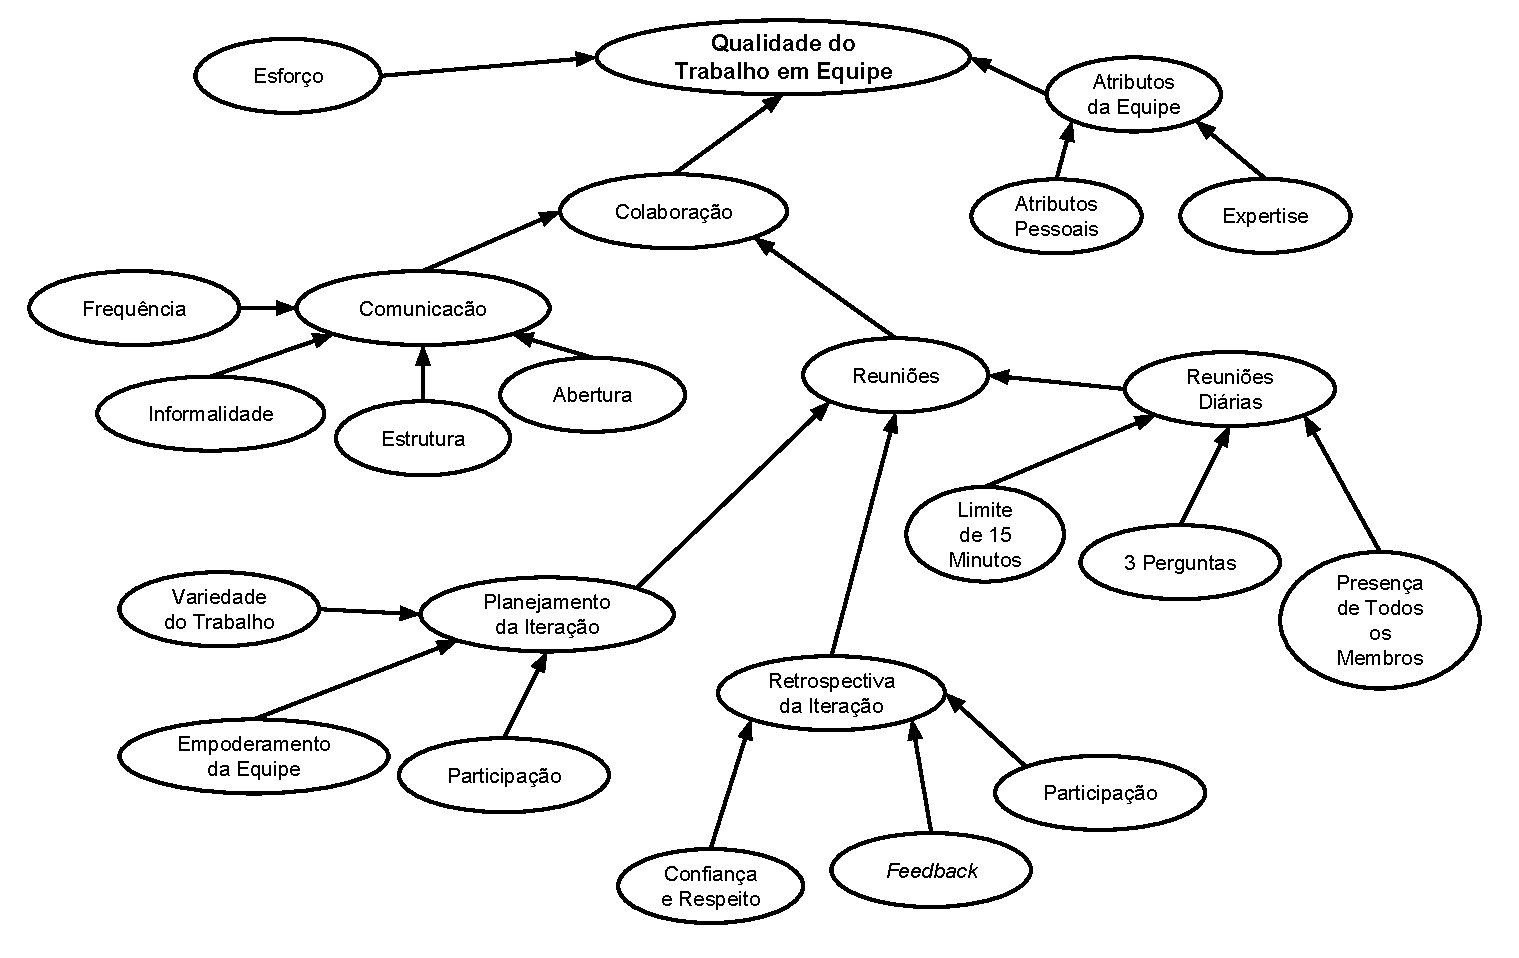
\includegraphics[scale=0.6]{figs/modeloSBES.pdf}}
    \end{center}
    \caption{Modelo Proposto no Trabalho Base}
    \label{trabalho:base:modelo}
\end{figure}

As tabelas de probabilidade desse modelo foram definidas utilizando o método de \cite{perkusichNPT}. Contudo, em vez de utilizar \textit{surveys} online, foram realizadas entrevistas com o mesmos especialistas responsáveis por construir o GAD. Para cada nó filho presente no GAD, pediu-se que os especialistas ordenassem seus nós pai com base na sua relevância para o nó filho. Em seguida, com base nessas ordens de relevância foram definidas as expressões ponderadas para, finalmente, definir as TPN dos nós filho.

A validação desse modelo foi feita com simulação de cenários, e, de acordo com as conclusões, o modelo é uma boa representação do mundo real. Além disso, também foi concluído que o modelo permite que, baseado nos resultados do modelo, os indivíduos que o utilizam identifiquem problemas que compromentem a qualidade do TE. Entretanto, há alguns fatores que afetam a sua validade. São eles:

\begin{itemize}
  \item A utilização de apenas um trabalho como base para o modelo;
  \item A definição das TPN utilizando o método de Perkusich et al. utiliza apenas a função de média ponderada. Logo, as TPN de alguns nós podem estar inconsistentes pelo fato de sua definição ser restrita à essa função;
  \item O modelo não foi validado em projetos reais.
\end{itemize}

Portanto, nesta pesquisa, foi dada continuidade ao trabalho apresentado em \cite{freire}, buscando eliminar esses fatores que ameaçaram a sua validade.

\chapter{Apresentação do Modelo}
\label{modelo}

Conforme explicado na Seção \ref{fundamentacao:redes:construcao}, a construção de uma \textit{Rede Bayesiana} pode ser dividada em duas fases: a construção do GAD, e a definição das funções de probabilidade. Portanto, neste capítulo, serão descritas essas duas fases do processo de construção do modelo proposto neste trabalho. À princípio, será explicado como foram identificados os relacionamentos entre os fatores-chave do modelo. Em seguida, será descrito o processo adotado para a definição das funções de probabilidade, e porque foi decidido utilizar funções de probabilidade em vez de tabelas de probabilidade.

\section{Construção do GAD}
\label{modelo:gad}

Nesta fase da construção do modelo é necessário identificar os fatores-chave que influenciam a qualidade do TE de equipes ágeis e os relacionamentos entre esses fatores. Como base para a construção do GAD, optou-se por utilizar o modelo proposto em \cite{freire} (Figura \ref{modelo:gad:freire}). De acordo com os autores, o modelo apresentado é uma boa representação do mundo real. Entretanto, uma de suas limitações é que ele foi construído com base em apenas um trabalho. Assim, a partir desse modelo e dos fatores descritos na Seção \ref{fundamentacao:ageis:fatores}, é possível refinar o GAD, e, assim, obter uma representação mais fiel ao mundo real.

\begin{figure}[ht!]
\begin{center}
		\fbox{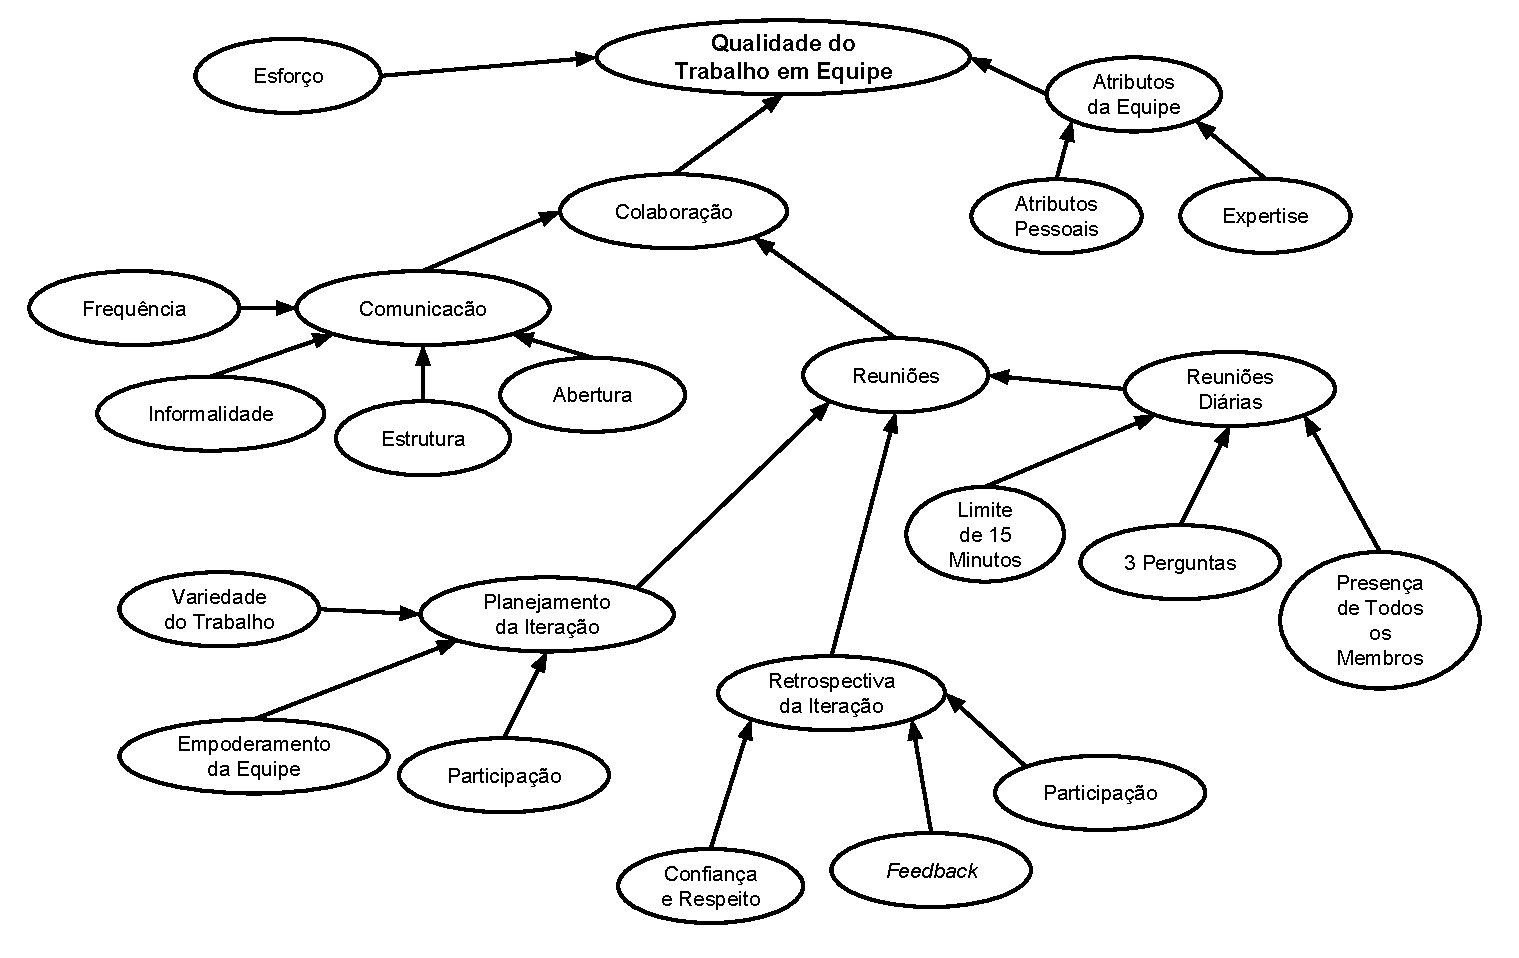
\includegraphics[scale=0.6]{figs/modeloSBES.pdf}}
	\end{center}
	\caption{Modelo Proposto por Freire et al.}
	\label{modelo:gad:freire}
\end{figure}

No modelo apresentado em \cite{freire}, a qualidade do TE depende diretamente de três principais nós: \textit{Colaboração}, \textit{Esforço} da equipe de desenvolvimento e \textit{Atributos da Equipe}. Entretanto, como foi decidido considerar o TE no contexto das relações entre os membros da equipe para alcançar os objetivos propostos, o nó \textit{Esforço} não se enquadra no contexto deste trabalho. Como é esperado que as equipes ágeis sejam auto-organizáveis \cite{manifesto}, o nó \textit{Esforço} foi substituído por \textit{Auto-Gerenciamento}. Dessa forma, o fator principal, \textit{Trabalho em Equipe}, passa a depender diretamente dos nós: \textit{Colaboração}, \textit{Auto-Gerenciamento} e \textit{Atributos da Equipe} (Figura \ref{modelo:gad:altonivel}).

\begin{figure}[ht!]
\begin{center}
		\fbox{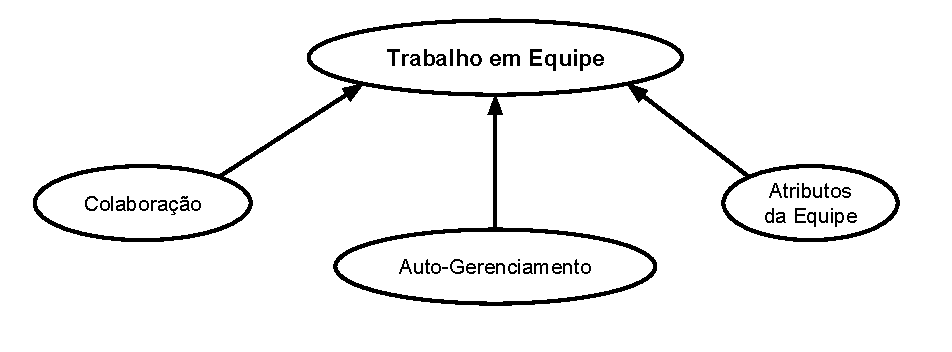
\includegraphics[scale=0.9]{figs/modeloAltoNivel.pdf}}
	\end{center}
	\caption{Representação do modelo proposto em alto nível.}
	\label{modelo:gad:altonivel}
\end{figure}

No modelo tomado como base, o nó \textit{Colaboração} depende diretamente dos nós \textit{Comunicação} e \textit{Reuniões}. \textit{Comunicação}, por sua vez, depende diretamente dos seguintes nós: \textit{Frequência}, \textit{Informalidade}, \textit{Estrutura} - possibilidade dos membros da equipe se comunicarem diretamente uns com os outros - e \textit{Abertura}, que está relacionada com o ato de não haver contenção de informação entre os membros da equipe. Como forma de minimizar a complexidade dos cálculos efetuados \cite{} e o viés que pode ser introduzido em virtude da subjetidade que esse nós representam, optou-se por substituir esses quatro nós por \textit{Distribuição da Equipe} e \textit{Cara-a-Cara}. Esse nós estão relacionados, respectivamente, com o fato dos membros da equipe compartilharem a mesma localidade e conversarem cara-a-cara diariamente. Dessa forma, a \textit{Distribuição da Equipe} substitui a \textit{Frequência}, uma vez que o fato de os membros da equipe compartilharem o mesmo local facilita a comunicação \cite{lalsing} e, assim, contribui para que a comunicação ocorra em maior frequência. Já o nó \textit{Cara-a-Cara} substitui a \textit{Informalidade}, \textit{Estrutura} e \textit{Abertura}, tendo em vista que essa prática contribui para que essas características se façam na presentes na \textit{Comunicação}.

O nó \textit{Reuniões}, que no modelo base depende diretamente dos nós \textit{Planejamento da Iteração}, \textit{Retrospectiva da Iteração} e \textit{Reuniões Diárias} foi substituído apenas pelo nó \textit{Reuniões Diárias}. Essa decisão foi tomada porque o que ocorre na \textit{Retrospectiva da Iteração} não influenciará mais o TE na iteração que se passou. O \textit{Planejamento da Iteração}, por sua vez, está relacionado com a utilização de técnicas de Engenharia de \textit{Software} que facilitam na prevenção contra riscos e estimativa de tempo para cumprimento de atividades. Além disso, não é objetivo do \textit{Planejamento da Iteração} melhorar a \textit{Comunicação} e a \textit{Colaboração} das equipes.

Conforme descrito em \cite{freire}, o nó \textit{Reuniões Diárias} depende diretamente dos seguintes nós: \textit{Limite de 15 Minutos}, \textit{3 Perguntas} (i.e., "O que eu fiz hoje?", "O que farei amanhã?" e "Quais obstáculos estão impedindo o meu progresso?") e \textit{Presença de Todos os Membros}. Entretanto, de acordo com Moe et al. \cite{moe2}, é necessário aplicar o \textit{Monitoramento} para que os membros da equipe observem as atividades e a eficiência dos outros integrantes, além de reconhecerem quando um membro da equipe atua corretamente, provendo \textit{feedback} e apoio. Logo, como o objetivo das perguntas é permitir aos participantes identificar potenciais barreiras e manter a coordenação da equipe, e isso está relacionando com o \textit{Monitoramento}, decidiu-se renomear o nó \textit{3 Perguntas} para \textit{Monitoramento}. Além disso, as três perguntas as quais o nó está relacionado são referentes ao contexto de \textit{Scrum}, e o modelo proposto neste trabalho é para avaliação do TE de equipes ágeis em geral. Também foi decidido remover o nó \textit{Limite de 15 minutos} porque ele não é considerado um indicador de qualidade dessas reuniões.

Em \cite{moe}, são descritos cinco fatores que precisam ser levados em conta para melhorar o TE de equipes ágeis. São eles: \textit{Liderança Compartilhada}, \textit{Orientação da Equipe}, \textit{Redundância}, \textit{Aprendizagem da Equipe} e \textit{Autonomia da Equipe}. A seguir, há a definição de cada um desses fatores com base nesse trabalho anteriormente citado:

\begin{itemize}
  \item \textit{Liderança Compartilhada}: Todos os membros da equipe compartilham a autoridade das decisões em vez centralizá-la. Dessa forma, evita que apenas uma pessoa tome as decisões, ou todos os membros da equipe tomem decisões levando em consideração apenas o seu trabalho individual, independente dos outros membros da equipe. Geralmente, o indivíduo que possui o conhecimento necessário durante uma determinada fase do projeto assume a liderança, compartilhando os seus conhecimentos, e permitindo que todos participem do processo de tomada de decisões;
  \item \textit{Orientação da Equipe}: Priorização dos objetivos da equipe em vez dos objetivos indivíduais, respeitando o compartamento de cada um dos membros da equipe;
  \item \textit{Redundância}: Os membros da equipe podem substituir uns aos outros sem treinamento extenso;
  \item \textit{Aprendizagem da Equipe}: Melhoria contínua dos métodos de trabalho com base nos \textit{feedbacks} fornecidos à equipe;
  \item \textit{Autonomia da Equipe}: As decisões tomadas pela equipe são respeitadas pelos gerentes que estão fora dela.
\end{itemize}

Ainda sobre as \textit{Reuniões Diárias}, durante elas, os membros da equipe tem a possibilidade de regular seus limites e condições, escolhendo em quais atividades desejam trabalhar, além de negociar e discutir sobre prevenção contra riscos e medidas corretivas. Como isso está relacionado à \textit{Autonomia da Equipe}, também foi decidido adicioná-lo como nó que influencia as \textit{Reuniões Diárias}. Dessa forma, tem-se que as \textit{Reuniões Diárias} tornam-se diretamente dependentes de \textit{Monitoramento}, \textit{Presença de Todos os Membros} e \textit{Autonomia da Equipe}.

Além disso, conforme supracitado, pode-se concluir que a \textit{Orientação da Equipe} contribui diretamente para a \textit{Colaboração} da equipe, pois há uma preocupação em priorizar os objetivos da equipe em vez dos objetivos individuais. Dessa forma, é necessário que os membros da equipes trabalhem de forma coesa, colaborando para que os objetivos da equipe sejam sempre alcançados. Por isso, decidiu-se adicionar o nó \textit{Orientação da Equipe} como influenciate do nó \textit{Colaboração}. Com isso, conforme representado na Figura \ref{modelo:gad:colaboracao}, o nó \textit{Colaboração} passa a depender diretamente dos nós \textit{Comunicação}, \textit{Orientação da Equipe} e \textit{Reuniões Diárias}.

\begin{figure}[ht!]
\begin{center}
		\fbox{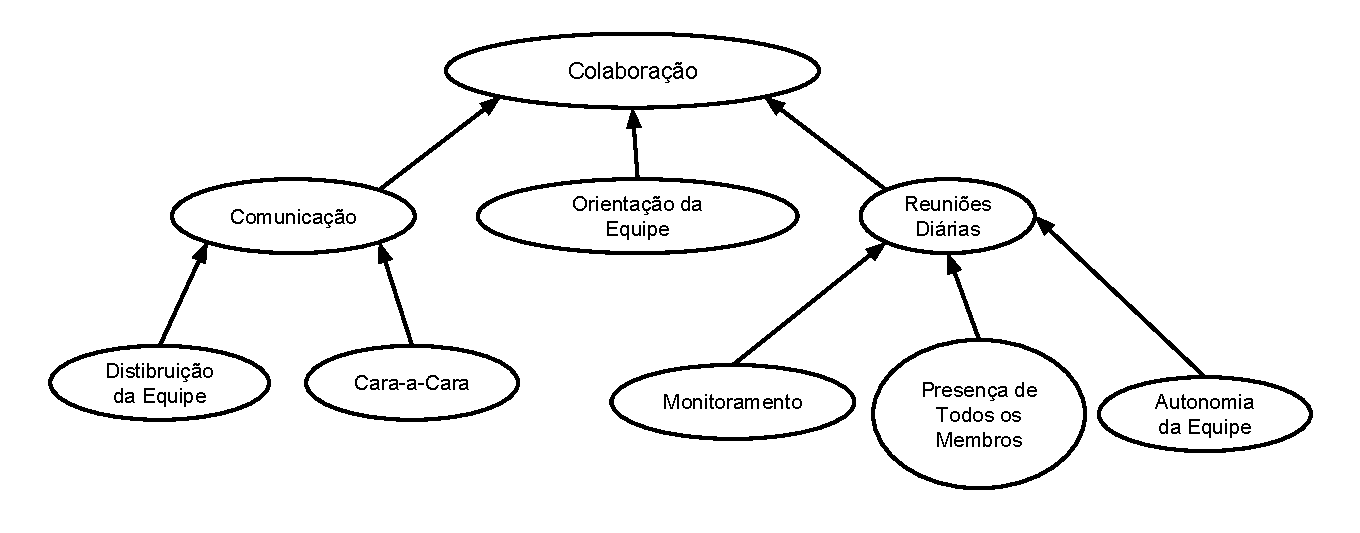
\includegraphics[scale=0.68]{figs/modeloColaboracao.pdf}}
	\end{center}
	\caption{Colaboração e os fatores que a influenciam.}
	\label{modelo:gad:colaboracao}
\end{figure}

\textit{Auto-Gerenciamento} é um dos novos nós que foi adicionado ao modelo, e influencia diretamente o TE. Na literatura, é estabelecido que a autoridade da decisão e da liderança de equipes auto-organizáveis precisa ser compartilhada \cite{morgan} \cite{kirkman}. Além disso, ainda em \cite{morgan}, é dito que equipes auto-organizáveis requerem uma capacidade de aprendizagem das equipes para que elas possam adaptar-se às transformações que ocorrem no ambiente. Ainda de acordo com \cite{morgan}, toda equipe que possui a capacidade de se auto-gerenciar precisa de um certo grau de \textit{Redundância}. Logo, com base nessas afirmações, os nós \textit{Liderança Compartilhada}, \textit{Aprendizagem da Equipe} e \textit{Redundância} foram adicionados como pais do nó \textit{Auto-Gerenciamento}. Na Figura \ref{modelo:gad:autogerenciamento} está representado o nó \textit{Auto-Gerenciamento} em conjunto com seus nós pai.

\begin{figure}[ht!]
\begin{center}
		\fbox{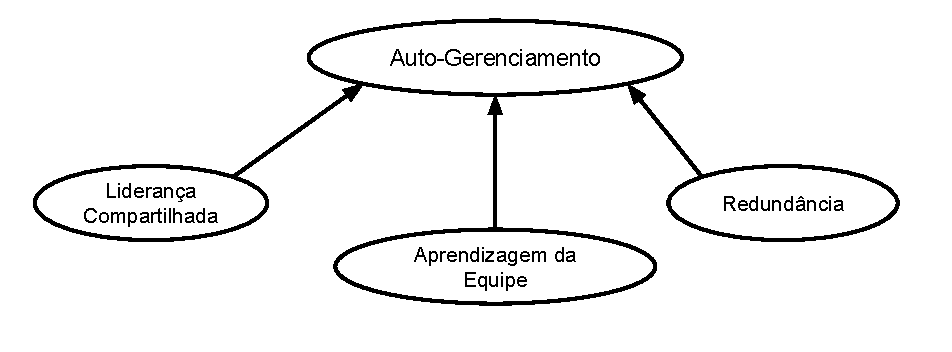
\includegraphics[scale=0.9]{figs/modeloAutoGerenciamento.pdf}}
	\end{center}
	\caption{Auto-Gerenciamento e os fatores que o influenciam.}
	\label{modelo:gad:autogerenciamento}
\end{figure}

O nó \textit{Atributos da Equipe} foi mantido como proposto no modelo em \cite{freire}. A Figura \ref{modelo:gad:atributos} contém a representação gráfica desse nó em particular.

\begin{figure}[ht!]
\begin{center}
		\fbox{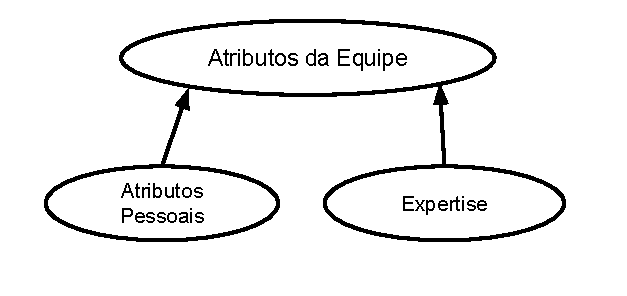
\includegraphics[scale=0.9]{figs/modeloAtributos.pdf}}
	\end{center}
	\caption{Atributos da Equipe e os fatores que o influenciam.}
	\label{modelo:gad:atributos}
\end{figure}

Finalmente, após definir os nós do GAD e os relacionamentos entre eles, na Figura \ref{modelo:gad:final} é possível verificar o GAD completo.

\begin{figure}[ht!]
\begin{center}
		\fbox{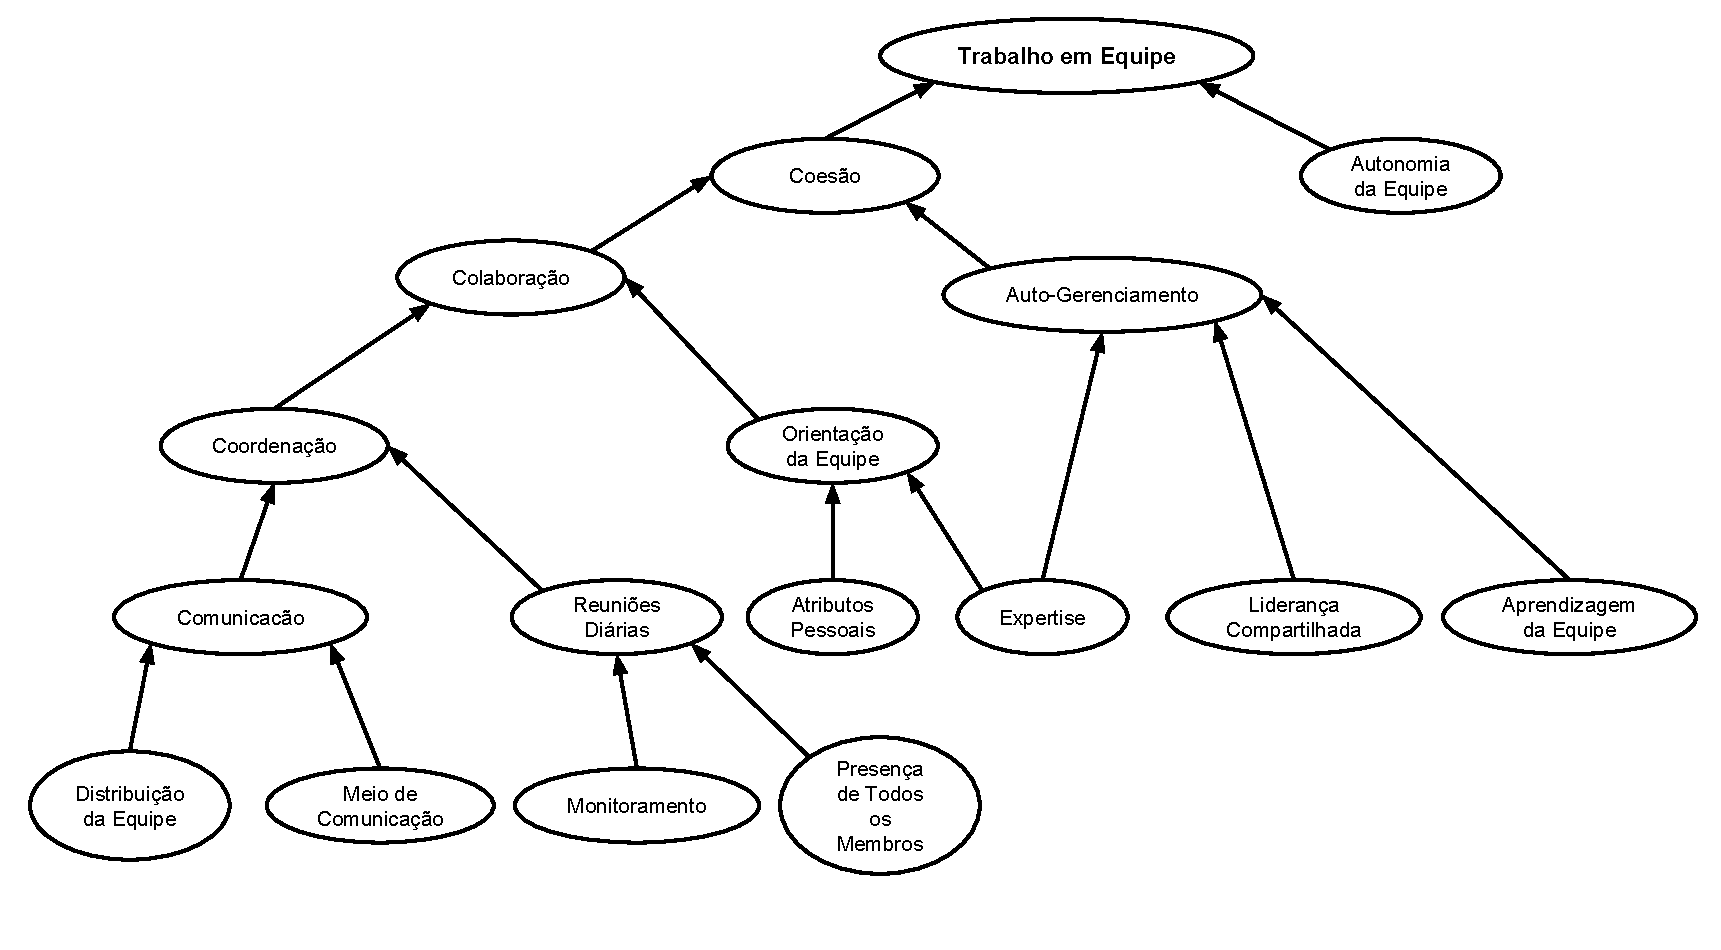
\includegraphics[scale=0.57]{figs/modeloFinal.pdf}}
	\end{center}
	\caption{Estrutura final do modelo proposto.}
	\label{modelo:gad:final}
\end{figure}

\section{Definição das Funções de Probabilidade}
\label{modelo:funcoes}

Apesar de \textit{Redes Bayesianas} serem um úteis para resolverem problemas reais relacionados com risco e subjetividade, o seu uso ainda é restrito devido a dificuldade em definir as TPN. Há duas maneiras de se coletar dados para definir as TPN de uma \textit{Rede Bayesiana}: base de dados ou opinião de especialistas. Contudo, não é fácil encontrar uma base de dados adequada para um cenário específico de um problema prático. Por outro lado, a definição das TPN com a ajuda de especialistas requer bastante esforço (e.g., definir TPN para nós com um número muito alto de estados ou alta quantidade de pais, pois a quantidade de linhas de uma TPN aumenta exponencialmente em função da quantidade de pais do nó em questão). De acordo com Fenton et al. \cite{fenton}, isso pode acarretar em vários tipos de inconsistências no modelo.

Há vários métodos que têm como objetivo diminuir a complexidade e para codificar a experiência em grandes TPN. Noisy-OR \cite{huang} e Noisy-MAX \cite{diez} são dois métodos bem estabelicidos. Contudo, Noisy-OR só pode ser aplicado a nós booleanos, e Noisy-MAX não é capaz de modelar o intervalo de relacionamentos que precisamos neste trabalho. Das \cite{das} propôs um algoritmo para popular as TPN que visa diminuir o tempo de duração para adquirir conhecimento de especialistas. Perkusich et al. \cite{perkusichNPT}, por sua vez, propõem um algoritmo cujo objetivo é ordenar os nós pai dadas as suas magnitudes relativas para o nó filho. Em seguida, com os nós filho ordenados, deve-se gerar as funções ponderadas com base na relevância dos nós pais e, finalmente, aplicá-las como funções de probabilidade dos nós.

Por outro lado, Fenton et al. \cite{fenton} propõem uma abordagem para \textit{Redes Bayesianas} que faz utiliza \textit{Nós Ranqueados}. Essa abordagem é baseada numa distribuição normal duplamente truncada (TNormal) que usa como média um tipo de função ponderada em função dos valores dos nós pai. Essa distribuição é baseada em quatro parâmetros: $u$, média (i.e., tendência central); $\sigma^{2}$, variância (i.e., confiança dos resultados); $a$, limite inferior (i.e., 0); e $b$, limite superior (i.e., 1). Essa distribuição permite que quem a utilize modele uma varidade de formas (i.e., relacionamentos. Por exemplo: uma distribuição uniforme ($\sigma^{2} = \infty$) e distribuições muito enviesadas ($\sigma^{2} = 0$). Na Figura \ref{modelo:funcoes:tnormal} há alguns exemplos de funções TNormal.


%\begin{figure}[ht!]
%\begin{center}
%		\fbox{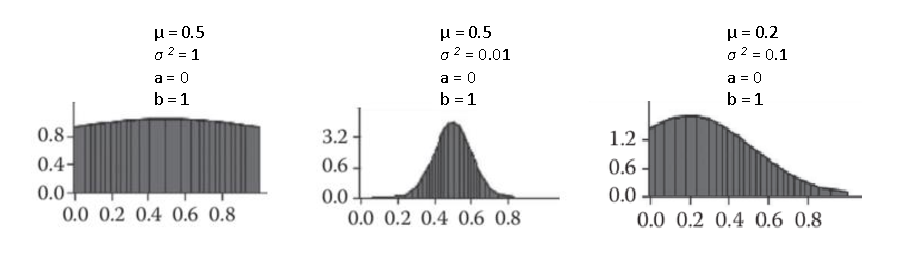
\includegraphics[scale=0.57]{figs/tnormalExemplos.pdf}}
%	\end{center}
%	\caption{Exemplos de Funções TNormal.}
%	\label{modelo:funcoes:tnormal}
%\end{figure}

Nessa abordagem, $u$ é definido por uma função ponderada baseada nos nós pai. Existem quatro tipos de funções ponderadas: média ponderada (WMEAN), mínimo ponderada (WMIN), máximo ponderada (WMAX) e uma mistura da função WMIN e WMAX (MIXMINMAX). De acordo com os autores, essas funções são suficientes para representar os tipos de relações necessárias para definir as TPN. A Figura \ref{modelo:funcoes:ponderadas} contém exemplos de TPN calculadas com essas funções. Entretanto, apesar de WMEAN e MIXMINMAX apresentarem os mesmos valores, há uma diferença entre elas. A função WMEAN calcula a média ponderada dos nós pai, baseado nos pesos de cada nó pai, e a função MIXMINMAX mescla as funções WMIN e WMAX, também baseado nos pesos dos nós pai.

%\begin{figure}[ht!]
%\begin{center}
%		\fbox{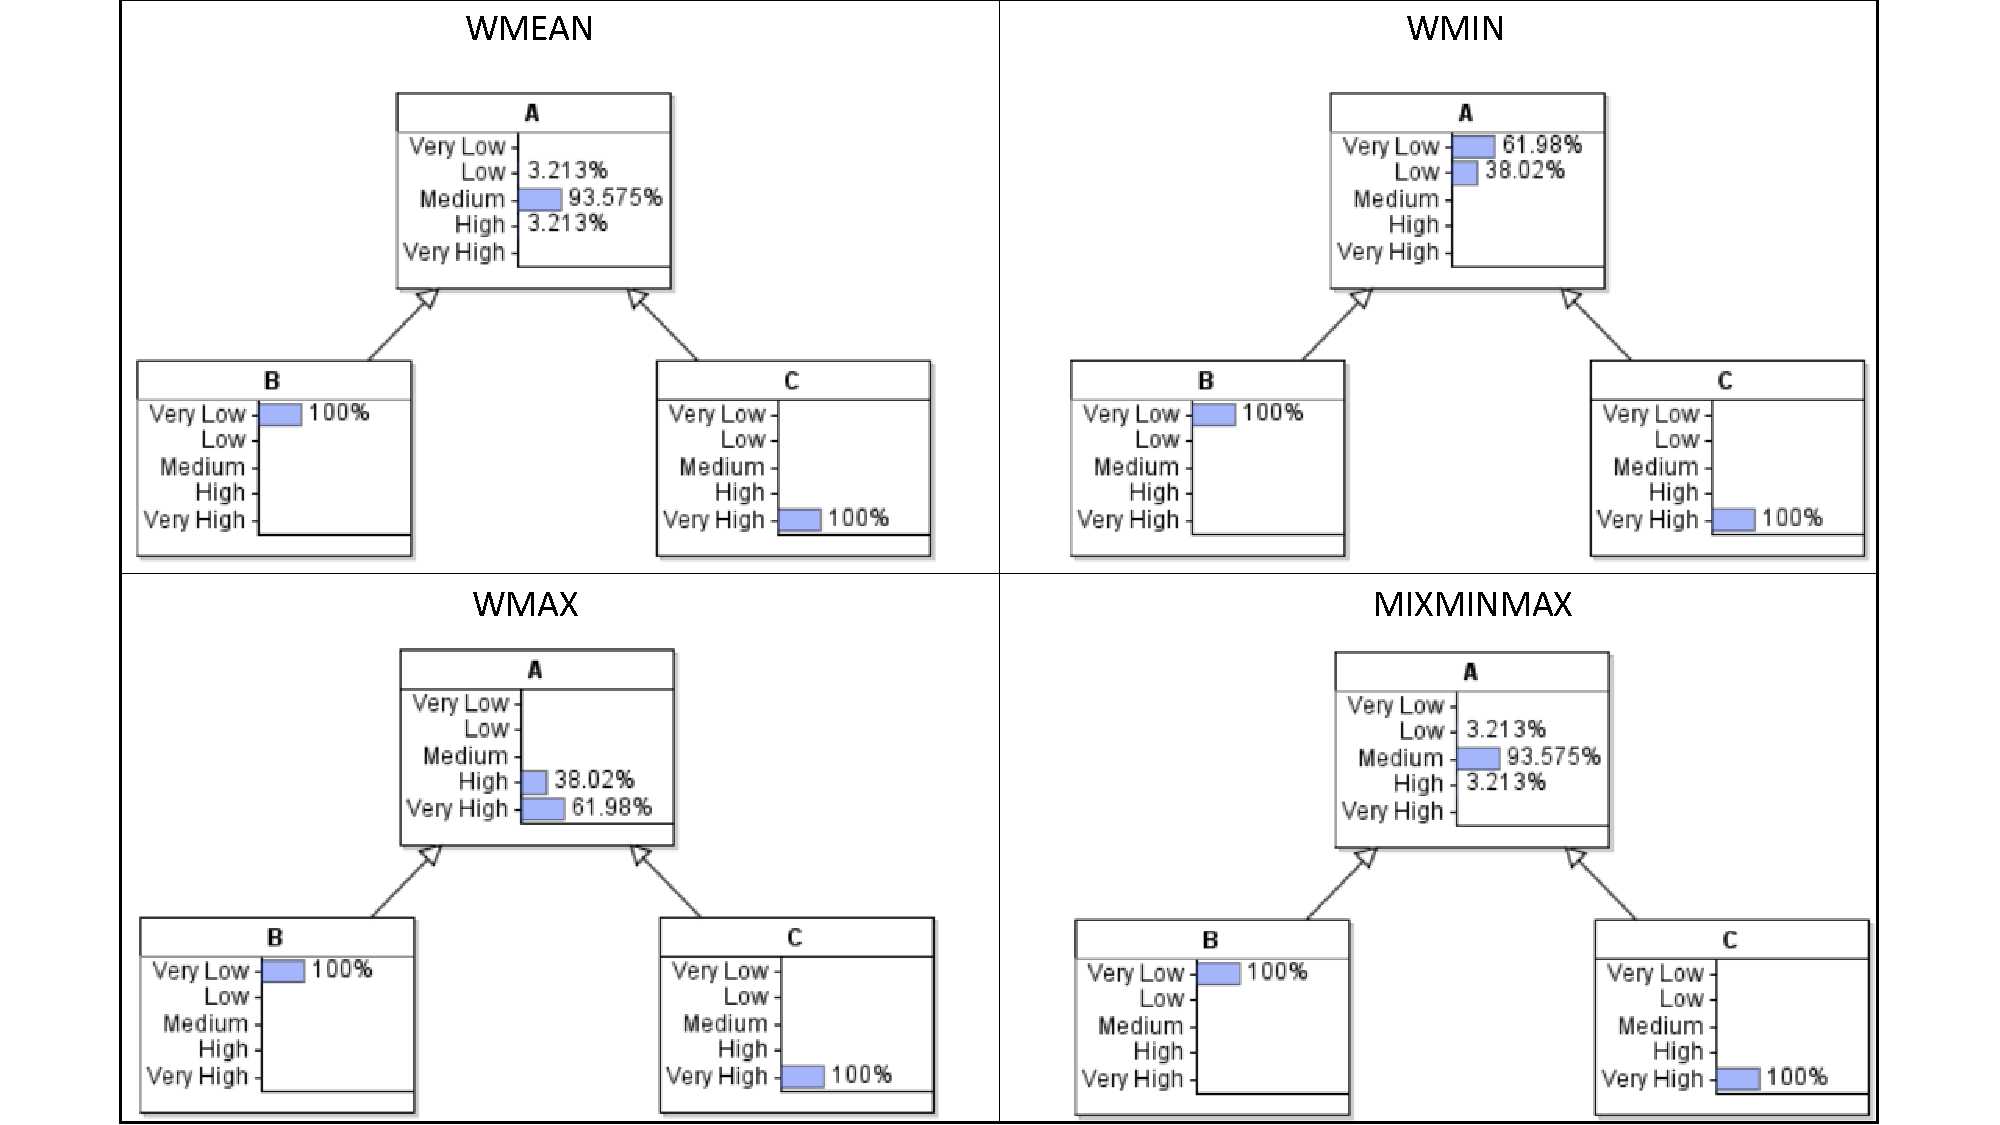
\includegraphics[scale=0.57]{figs/funcoesExemplos.pdf}}
%	\end{center}
%	\caption{Exemplos das Funções Ponderadas.}
%	\label{modelo:funcoes:ponderadas}
%\end{figure}

Para definir qual função deve ser utilizada, o indivíduo que está construindo o modelo deve definir perguntas para coletar respostas e definir as TPN. Tomando como base a \textit{Rede Bayesiana} representada na Figura \ref{modelo:funcoes:bn1}, um exemplo de pergunta seria: "Se o nó X1 for Muito Alto e o nó X2 for Muito Baixo, qual o valor esperado para o nó Y?". Baseado nas respostas, o indivíduo que está construindo a \textit{Rede Bayesiana} deve definir qual a função e quais o pesos para adequados para definir as TPN. A variância deve ser definida empiricamente e deve refletir a confiança dos especialistas nos resultados.

\begin{figure}[ht!]
\begin{center}
		\fbox{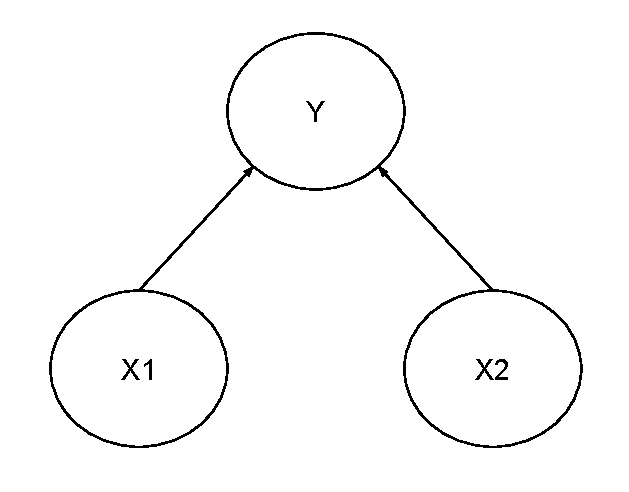
\includegraphics[scale=0.8]{figs/BN-2nos.pdf}}
	\end{center}
	\caption{Exemplo de nó filho com dois pais.}
	\label{modelo:funcoes:bn1}
\end{figure}

Entretanto, a base da abordagem proposta em \cite{fenton} consiste em mapear os estados dos nós em uma escala numérica. Logo, quanto menos precisa a tendência central do nó filho, mais vaga será a distribuição da função atribuida. Como forma de mitigar esses problemas, em \cite{laitila} é proposta uma abordagem similar. Contudo, nessa abordagem, em vez do especialista avaliar a função de probabilidade de um determinado nó filho atribuindo a qual dos estados desse nó a tendência central corresponde, são atríbuidas probabilidades para cada um dos estados do nó filho - a soma dessas probabilidades deve ser igual a 1. De acordo com os autores, essa abordagem provê uma transparência maior na elicitação dos pesos dos nós pai na função ponderada. Portanto, decidiu-se utilizar essa abordagem para definir as funções de probabilidade do modelo proposto.

Um especialista em \textit{Redes Bayesianas} e Métodos Ágeis foi o responsável por realizar essa atividade. Para cada nó filho, o especialista deve definir quais as probabilidades desse nó estar em cada estado, com base nos estados dos nós pai. Portanto, para um nó com dois pais, e tomando como exemplo a \textit{Rede Bayesiana} apresentada na Figura \ref{modelo:funcoes:bn1}, o especialista precisou preencher as células em branco da Tabela \ref{modelo:funcoes:tabela2nos} com os valores esperados, de forma que, para cada combinação possível

\begin{align}
  \sum_{i=1}^{n}Pi = 1,\\ \intertext{onde $Pi$ é a probabilidade de cada estado e $n$ é a quantidade de estados possíveis do nó filho}
\end{align}

\begin{table}[ht!]
\centering
\caption{Tabela para definição das Funções de Probabilidade de nós com dois pais}
\label{modelo:funcoes:tabela2nos}
\begin{tabular}{|c|c|c|c|c|c|c|}
\hline
\multicolumn{2}{|l|}{}                      & \multicolumn{5}{c|}{\textbf{Valores Esperados para Y}}                                       \\ \hline
\textbf{X1}          & \textbf{X2}          & \textbf{Muito Baixa} & \textbf{Baixa} & \textbf{Média} & \textbf{Alta} & \textbf{Muito Alta} \\ \hline
\textbf{Muito Alta}  & \textbf{Muito Baixa} & $P_{1}$              & $P_{2}$        & $P_{3}$        & $P_{4}$       & $P_{5}$              \\ \hline
\textbf{Muito Baixa} & \textbf{Muito Alta}  & $P_{1}$              & $P_{2}$        & $P_{3}$        & $P_{4}$       & $P_{5}$             \\ \hline
\textbf{Muito Alta}  & \textbf{Média}       & $P_{1}$              & $P_{2}$        & $P_{3}$        & $P_{4}$       & $P_{5}$             \\ \hline
\textbf{Média}       & \textbf{Muito Alta}  & $P_{1}$              & $P_{2}$        & $P_{3}$        & $P_{4}$       & $P_{5}$             \\ \hline
\end{tabular}
\end{table}

De maneira análoga, para cada nó filho com três pais (e.g., Figura \ref{modelo:funcoes:bn2}), porém com uma maior quantidade de combinações possíveis, o especialista precisou preencher as células em branco de uma similar à Tabela \ref{modelo:funcoes:tabela3nos}.

\begin{figure}[ht!]
\begin{center}
		\fbox{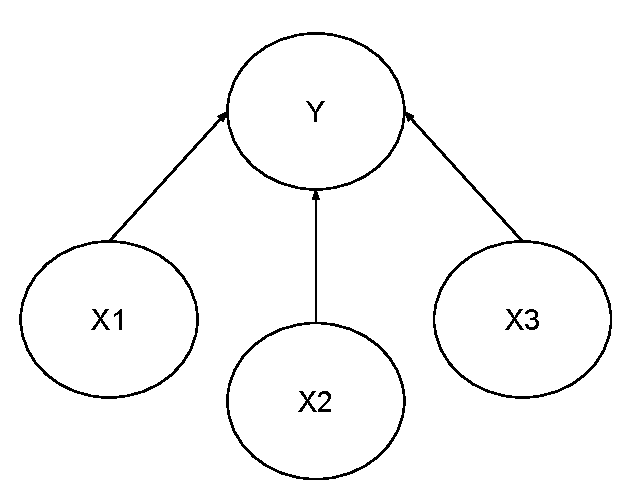
\includegraphics[scale=0.8]{figs/BN-3nos.pdf}}
	\end{center}
	\caption{Exemplo de nó filho com três pais.}
	\label{modelo:funcoes:bn2}
\end{figure}

\begin{table}[ht!]
\centering
\caption{Tabela para definição das Funções de Probabilidade de nós com três pais}
\label{modelo:funcoes:tabela3nos}
\resizebox{\textwidth}{!}{\begin{tabular}{|c|c|c|c|c|c|c|c|}
\hline
\multicolumn{3}{|c|}{}                                             & \multicolumn{5}{c|}{\textbf{Valores Esperados para Y}}                                       \\ \hline
\textbf{X1}          & \textbf{X2}          & \textbf{X3}          & \textbf{Muito Baixa} & \textbf{Baixa} & \textbf{Média} & \textbf{Alta} & \textbf{Muito Alta} \\ \hline
\textbf{Muito Alta}  & \textbf{Muito Alta}  & \textbf{Muito Baixa} & $P_{1}$              & $P_{2}$        & $P_{3}$        & $P_{4}$       & $P_{5}$              \\ \hline
\textbf{Muito Alta}  & \textbf{Muito Baixa} & \textbf{Muito Alta}  & $P_{1}$              & $P_{2}$        & $P_{3}$        & $P_{4}$       & $P_{5}$              \\ \hline
\textbf{Muito Baixa} & \textbf{Muito Alta}  & \textbf{Muito Alta}  & $P_{1}$              & $P_{2}$        & $P_{3}$        & $P_{4}$       & $P_{5}$              \\ \hline
\textbf{Muito Baixa} & \textbf{Muito Baixa} & \textbf{Muito Alta}  & $P_{1}$              & $P_{2}$        & $P_{3}$        & $P_{4}$       & $P_{5}$              \\ \hline
\textbf{Muito Baixa} & \textbf{Muito Alta}  & \textbf{Muito Baixa} & $P_{1}$              & $P_{2}$        & $P_{3}$        & $P_{4}$       & $P_{5}$              \\ \hline
\textbf{Muito Alta}  & \textbf{Muito Baixa} & \textbf{Muito Baixa} & $P_{1}$              & $P_{2}$        & $P_{3}$        & $P_{4}$       & $P_{5}$              \\ \hline
\end{tabular}}
\end{table}

Assim, de acordo com a quantidade de nós pai de um determinado nó, foram definidas tabelas para cada um dos nós presentes no modelo proposto, exceto os nós de entrada. Uma vez que essas tabelas foram definidas, o especialista, com a ajuda de uma ferramenta, calculou os resultados reais para cada estado. Esses cálculos foram feitos diversas vezes, pois há a necessidade de definir qual função ponderada representa a tabela de probabilidade do nó em questão, além dos pesos de cada um dos nós pai praquela função. Esses cálculos são realizados diversas vezes até que a função e os pesos adequados, que mais se aproximem dos valores esperados, sejam encontrados. Além disso, o processo de definição das funções de probabilidade por parte do especialista é muito importante, pois caso haja inconsistências na definição do GAD, é necessário reorgarnizar a estrutura do grafo para garantir a consistência entre os conceitos e relacionamentos que estão sendo representados. Finalmente, ao final desse processo, o modelo está pronto para ser utilizado. A Tabela \ref{modelo:funcoes:tabelapesos} contém as funções e os pesos dos nós pai de todos os nós do modelo, exceto os nós de entrada.

\begin{table}[ht!]
\centering
\caption{Definição das Funções de Probabilidade}
\label{modelo:funcoes:tabelapesos}
\resizebox{\textwidth}{!}{\begin{tabular}{|c|c|c|c|c|c|c|c|c|}
\hline
\multicolumn{3}{|c|}{\textbf{}}                                                                                                      & \multicolumn{3}{c|}{\textbf{Pais}}                                                                                                                                                                            & \multicolumn{3}{c|}{\textbf{Pesos}}                                      \\ \hline
\textbf{Nó}                                                              & \textbf{Função} & \multicolumn{1}{l|}{\textbf{Variância}} & \textbf{Pai 2}                                                    & \textbf{Pai 2}                                                         & \textbf{Pai 3}                                                   & \textbf{Peso do Pai 1} & \textbf{Peso do Pai 2} & \textbf{Peso do Pai 3} \\ \hline
\textbf{Trabalho em Equipe}                                              & wmin            & 0,0005                                  & Colaboração                                                       & Auto-Gerenciamento                                                     & \begin{tabular}[c]{@{}c@{}}Autonomia \\ da Equipe\end{tabular}   & 10                     & 10                     & 10                     \\ \hline
\textbf{Colaboração}                                                     & wmin            & 0,0005                                  & Comunicação                                                       & Reuniões Diárias                                                       & \begin{tabular}[c]{@{}c@{}}Orientação \\ da Equipe\end{tabular}  & 10                     & 10                     & 10                     \\ \hline
\textbf{Auto-Gerenciamento}                                              & wmin            & 0,0005                                  & Expertise                                                         & \begin{tabular}[c]{@{}c@{}}Liderança \\ Compartilhada\end{tabular}     & \begin{tabular}[c]{@{}c@{}}Aprendizagem\\ da Equipe\end{tabular} & 3                      & 2                      & 1                      \\ \hline
\textbf{Comunicação}                                                     & wmin            & 0,0005                                  & \begin{tabular}[c]{@{}c@{}}Distribuição \\ da Equipe\end{tabular} & \begin{tabular}[c]{@{}c@{}}Meio \\ de Comunicação\end{tabular}         & X                                                                & 3                      & 5                      & X                      \\ \hline
\textbf{Reuniões Diárias}                                                & wmin            & 0,0005                                  & Monitoramento                                                     & \begin{tabular}[c]{@{}c@{}}Presença de Todos\\ os Membros\end{tabular} & X                                                                & 7                      & 7                      & X                      \\ \hline
\textbf{\begin{tabular}[c]{@{}c@{}}Orientação \\ da Equipe\end{tabular}} & wmin            & 0,0005                                  & \begin{tabular}[c]{@{}c@{}}Atributos \\ Pessoais\end{tabular}     & Expertise                                                              & X                                                                & 5                      & 5                      & X                      \\ \hline
\end{tabular}}
\end{table}

\chapter{Descrição da Abordagem Proposta}
\label{descricao}

Como apresentado na Seção \ref{introducao:objetivos:especificos}, dois dos principais objetivos desta pesquisa são: Propor um modelo baseado em \textit{Redes Bayesianas} para avaliar o TE de equipes ágeis e uma abordagem para utilizar o modelo proposto. Portanto, para utilizar o modelo proposto no Capítulo \ref{modelo}, neste capítulo será descrita a abordagem proposta.

Essa abordagem é dividida em etapas que englobam desde a coleta dos dados para alimentação do modelo, até o processo de tomada de decisões preventivas e corretivas por parte dos gerentes de projeto. Além disso, propõe-se que essa aborgadem deve ser utilizada antes da reunião de \textit{Retrospectiva da Iteração} para que, durante essa reunião, os gerentes de projeto possam reportar os resultados obtidos para a equipe, além de auxiliar na tomada de decisões para a próxima iteração. Portanto, neste capítulo, serão descritas todas as etapas dessa abordagem. A Figura \ref{} contém o fluxo completo da abordagem e as interações entre as etapas.

{\color{red} Figura ilustrando o método...}

A primeira etapa da abordagem diz respeito à coleta de dados e alimentação dos modelos. As perguntas necessárias para coletar os dados referentes aos nós de entrada do modelo estão estão definidas no Apêndice \ref{questionarios}. Com isso, caso uma empresa/organização deseje avaliar o TE de suas equipes, ou um gerente de projeto em particular deseje fazê-lo individualmente, basta responder as perguntas referentes aos nós de entrada para, assim, obter os resultados calculados pelo modelo.

A segunda etapa consiste da análise dos resultados calculados pelo modelo. Como o fator principal para o qual o modelo calcula os resultados, \textit{Trabalho em Equipe}, é subjetivo, há muita dificuldade para calcular esse fator de forma objetiva. Contudo, o TE é um fator que tem influência sobre outros fatores que podem ser medidos de forma objetiva (e.g., FATOR A, FATOR B, FATOR C) \cite{}. Portanto, para facilitar a análise dos dados, propõe-se que os indivíduos que utilizam esta abordagem adotem os resultados calculados pelo modelo como indicadores de uma determinada métrica que represente um desses fatores que são influenciados pelo TE. Dessa forma, em vez de analisar os resultados calculados comparando-os com resultados esperados pelos gerentes de projeto, a análise será menos sujeita a viés. Entretanto, é necessário atentar para o fato de que o TE, possivelmente, não é o único fator que influencia o fator com o qual ele está sendo comparado. Logo, para realizar a análise dos dados, talvez seja necessário fazer algumas presunções, que podem afetar a validade dessa análise.

Baseado nos resultados calculados pelo modelo e pelas análises realizadas pelos gerentes de projeto, há a possibilidade de tomar medidas preventivas e corretivas para serem aplicadas nas iterações seguintes, garantindo, assim, a melhoria do TE e do produto e do processo como um todo.

Propõe-se que os indivíduos que desejem utilizar essa abordagem realizem esses três passos do início ao final do projeto, sempre ao final das iterações, para avaliar o TE das equipes na iteração que se passou. Além disso, também há a possibilidade de utilização dessa abordagem pare realizar predições. Essa aplicação é útil para que os gerentes de projeto possam avaliar tomar decisões preventivas antes do começo de um determinado de projeto, baseando-se na equipe com a qual ele irá trabalhar. Dessa forma, é possível diminuir os riscos referentes às interações entre os integrantes da equipe. 
\chapter{Estudo de Caso}
\label{estudodecaso}

Estudo de caso é uma metodologia de pesquisa adequada para estudar fenômenos contemporâneos em seu contexto natural \cite{runeson}. Com base nessa afirmação e na necessidade de avaliar o modelo proposto neste trabalho e sua utilização, foi realizado um estudo de caso no Laboratório de Sistemas Embarcados e Computação Pervasiva (Embedded Lab)\footnote{\url{http://www.embeddedlab.org/}}. O Embedded Lab está localizado na UFCG e foi escolhido em virtude das suas relações envolvendo a academia e a indústria.

Vários projetos são executados no Embedded Lab em parceria com empresas com o objetivo de desenvolver produtos de \textit{software}. Em todos os projetos do Embedded Lab com foco em desenvolvimento de \textit{software}, a metodologia para gestão e planejamento utilizada é o \textit{Scrum}. Portanto, o contexto no qual este estudo de caso foi realizado é o de indústria, com utilização de \textit{Scrum} como metodologia ágil adotada. Assim, os resultados e conclusões obtidos neste estudo de caso são referentes a esse contexto. O estudo de caso foi realizado em X projetos, onde cada um deles foi considerado uma unidade de análise. {\color{red} A duração foi de X dias.}

\section{\textit{Design} do Estudo de Caso}
\label{estudodecaso:design}

\subsection{Objetivos}
\label{estudodecaso:design:objetivos}

Para este estudo de caso, foram definidos dois principais objetivos:

\begin{enumerate}
  \item Verificar a fidelidade do modelo proposto para a avaliação do TE de equipes \textit{Scrum} com relação ao mundo real;
  \item Verificar a utilidade da abordagem para utilização do modelo em projetos \textit{Scrum}.
\end{enumerate}

\subsection{Objetos de Estudo}
\label{estudodecaso:design:objetos}

Os objetos de estudo são:

\begin{enumerate}
  \item O modelo proposto para representar o TE de equipes \textit{Scrum};
  \item A abordagem proposta para utilização do modelo.
\end{enumerate}

Logo, com base nos objetos de estudo definidos, deseja-se avaliar: a precisão do modelo proposto, a sua utilidade para auxiliar na liderança de equipes \textit{Scrum} e A facilidade de implementação e utilização da abordagem proposta.

\subsection{Questões de Pesquisa}
\label{estudodecaso:design:perguntas}

Com base nos objetivos definidos para este estudo de caso e visando alcançá-los, foram definidas as seguintes questões de pesquisa:

\begin{itemize}
  \item \textit{PP1}: O modelo proposto mensura de forma precisa o TE de equipes Scrum?
  \item \textit{PP2}: A utilização do modelo auxília na detecção de oportunidades de melhoria do TE de equipes Scrum?
  \item \textit{PP3}: A abordagem proposta é de fácil implementação e utilização?
  \item \textit{PP4}: O custo-benefício de utilizar a abordagem é positivo?
\end{itemize}

Dadas as questões de pesquisa definidas acima, as seguintes hipóteses foram definidas para respondê-las:

\begin{itemize}
  \item \textit{H0-1}: O modelo proposto não mensura de forma precisa o Trabalho em Equipe de equipes Scrum;
  \item \textit{HA-1}: O modelo proposto mensura de forma precisa o Trabalho em Equipe de equipes Scrum;
  \item \textit{H0-2}: A utilização do modelo não auxilia na detecção de oportunidades de melhoria do Trabalho em Equipe de equipes Scrum;
  \item \textit{HA-2}: A utilização do modelo auxilia na detecção de oportunidades de melhoria do Trabalho em Equipe de equipes Scrum;
  \item \textit{H0-3}: A abordagem proposta não é de fácil implementação e utilização;
  \item \textit{HA-3}: A abordagem proposta é de fácil implementação e utilização;
  \item \textit{H0-4}: O custo-benefício de utilizar a abordagem não é positivo;
  \item \textit{HA-4}: O custo-benefício de utilizar a abordagem é positivo.
\end{itemize}

Assim, \textit{H0-1} e \textit{HA-1} estão relacionadas à \textit{PP1}, \textit{H0-2} e \textit{HA-2} estão relacionadas à \textit{PP2}, \textit{H0-3} e \textit{HA-3} estão relacionadas à \textit{PP3}, e \textit{H0-4} e \textit{HA-4} estão relacionadas à \textit{PP4}.

\subsection{Unidades de Análise}
\label{estudodecaso:design:unidades}

\begin{longtable}{
|p{0.25\dimexpr \textwidth-3\arrayrulewidth-4\tabcolsep\relax}|
 p{0.25\dimexpr \textwidth-3\arrayrulewidth-4\tabcolsep\relax}|
 p{0.25\dimexpr \textwidth-3\arrayrulewidth-4\tabcolsep\relax}|
 p{0.25\dimexpr \textwidth-3\arrayrulewidth-4\tabcolsep\relax}|
}
\caption{Descrição das Unidades de Análise.\label{unidades}}\\

\hline
& \multicolumn{3}{|c|}{\textbf{Projeto}}\\
\hline
\multicolumn{1}{|c|}{\textbf{Característica}} & \textbf{A} & \textbf{B} & \textbf{C}\\
\hline
\endfirsthead

\hline
\multicolumn{4}{|c|}{Continuação da Tabela \ref{unidades}}\\
\hline
& \multicolumn{3}{|c|}{\textbf{Projeto}}\\
\hline
\multicolumn{1}{|c|}{\textbf{Característica}} & \textbf{A} & \textbf{B} & \textbf{C}\\
\hline
\endhead

\hline
\endfoot

\hline
% \multicolumn{2}{| c |}{End of Table}\\
% \hline\hline
% \endlastfoot

Experiência, em média de anos, dos integrantes da equipe participando em projetos de desenvolvimento de \textit{software} & 2.5 & 2 & 2 \\ \hline
Experiência, em média de anos, dos integrantes da equipe trabalhando em equipes ágeis & 1 & 1 & 2 \\ \hline
Breve descrição do cronograma do projeto & O cronograma inicial do projeto parecia ser tranquilo, mas como parte da equipe foi alocada para dar manutenção ao projeto anterior, acabou ficando mais apertado. & O projeto atual tem um cronograma que é relativamente fácil de alcançar, mas dependemos muito de outra entidade que está desenvolvendo o \textit{Hardware} que iremos trabalhar. & Cronograma sendo seguido no prazo, ficando apertado em alguns momentos. Algumas mudanças de requisitos geraram algum retrabalho, o que pode vir a comprometer algum item do cronograma inicial. \\ \hline
Breve descrição do escopo do projeto & Moderado. Os aplicativos a desenvolver são relativamente simples, mas a diversidade das plataformas suportadas contribui muito para a complexidade. & Uma ferramenta para monitoramento e controle de ativos de segurança patrimonial, é complexo. & Projeto de grande relevância para o cliente e complexo do ponto de vista de integração entre os componentes. O produto final depende da integração de componentes de \textit{software} e \textit{hardware} desenvolvidos por equipes do Embedded e do cliente. \\ \hline
Breve descrição da plataforma e tecnologias utilizadas no projeto & Plataforma: Desktop/Tablet (x86), Windows 8-10. Tecnologias: Visual Studio (com ReSharper), .NET / C\# e NUnit. & A plataforma utilizada no projeto é Android. Tecnologias utilizadas: SIP e RTSP. & Plataforma: Web. Tecnologias: Django e Python. \\ \hline

\end{longtable}

\subsection{Sujeitos - Quem utiliza a abordagem e o modelo?}
\label{estudodecaso:design:sujeitos}

Para cada unidade de análise, os sujeitos são líderes de projeto que atuam como \textit{Scrum Masters}. No Embedded Lab, esses sujeitos realizam atividades relacionadas ao processo e o gerenciamento da equipe, atividades relacionadas ao \textit{design} dos produtos, do ponto de vista gráfico e arquitetural de produto, além de implementação.

Na Tabela \ref{sujeitos}, são apresentados os perfis dos sujeitos em relação à experiência, em anos, desenvolvendo \textit{software}, liderando projetos de desenvolvimento, utilizando métricas no suporte à tomada de decisões e utilizando métodos ágeis.

\begin{table}[ht!]
\centering
\caption{Perfis dos Sujeitos.}
\label{sujeitos}
\resizebox{\textwidth}{!}{\begin{tabular}{|l|c|c|c|}
\hline
 & \multicolumn{3}{c|}{\textbf{Sujeito}} \\ \hline
\multicolumn{1}{|c|}{\textbf{Característica}}                                           & \textbf{1}  & \textbf{2} & \textbf{3} \\ \hline
Experiência, em anos, trabalhando em projetos de desenvolvimento de \textit{software}            & 5           & 10         & 10         \\ \hline
Experiência, em anos, liderando projetos de desenvolvimento de \textit{software}                 & 0.5         & 3          & 2          \\ \hline
Experiência, em anos, utilizando métricas e indicadores no suporte à tomada de decisões & 1.5         & 2          & 6          \\ \hline
Experiência, em anos, utilizando métodos ágeis                                          & 5           & 2          & 7          \\ \hline
\end{tabular}}
\end{table}

\subsection{Métodos}
\label{estudodecaso:design:metodos}

A coleta de dados é uma atividade necessária para responder as questões de pesquisas de um estudo de caso experimental. De acordo com Lethbridge et al. \cite{lethbridge}, há três diferentes categorias de métodos para coleta de dados: direto (e.g., entrevistas), indireto (e.g., \textit{survey}) e independente (e.g., análise de documentação). Portanto, o método utilizado para coleta de dados desse estudo de caso é o indireto, uma vez que os dados serão coletados por meio de questionários.

\subsection{Procedimento}
\label{estudodecaso:design:procedimento}

Neste estudo de caso, foi utilizada a ferramenta AgenaRisk para efetuar os cálculos do modelo. Em virtude de algumas limitações com licensas da ferramenta, o modelo foi criado e todos os cálculos realizados na máquina do pesquisador. Após a obtenção dos resultados, eles foram apresentados aos sujeitos em seguida pelo pesquisador. Após a definição do modelo, e dos questionários para avaliação do TE e da abordagem, este estudo de caso foi dividido em duas fases: \textit{Treinamento} e \textit{Utilização da Abordagem}.

\subsubsection{Fase 1 - Treinamento}
\label{estudodecaso:design:procedimento:treinamento}

O objetivo desta fase do estudo de caso é prover aos sujeitos o entendimento dos conceitos relacionados aos objetos de estudo. Assim, espera-se que ao final dessa fase qualquer dúvida em relação à esses fatores seja sanada para que os resultados não sejam influenciados por má-interpretação das perguntas dos questionários.

À princípio, os conceitos de \textit{Redes Bayesianas}, \textit{Ranked Nodes}, além de \textit{Funções de Probabilidade}, suas aplicações e funcionamento foram explicados para facilitar o entendimento da construção do modelo. Após isso, o modelo proposto nesta dissertação, e o relacionamento entre os fatores que o compõem foram explicados. Em seguida, foi explicado como seria realizado o processo de coleta de dados e quais perguntas do questionário de alimentação do modelo são referentes à quais nós de entrada do modelo. Por fim, foi explicado como é feita a análise dos resultados gerados pelo modelo, e como é possível identificar oportunidades de melhoria no TE. Alguns exemplos foram utilizados nessa fase para auxiliar no entendimento dos sujeitos.

\subsubsection{Fase 2 - Utilização da Abordagem}
\label{estudodecaso:design:procedimento:abordagem}



\subsection{Ameaças à Validade}
\label{estudodecaso:design:ameacas}

Runeson et al. \cite{runeson} afirmam que há diferentes maneiras de classificar aspectos da validade e ameaças à validade na literatura. No trabalho anteriormente citado, eles definem um esquema de classificação que distingue bem quatro aspectos da validade de um estudo de caso. São eles: \textit{Validade de Construção}, \textit{Validade Interna}, \textit{Validade Externa e Confiabilidade}.

O aspecto da \textit{Validade de Construção} está relacionado com o fato de o que é estudado realmente representar o que o pesquisador tem em mente estar de acordo com as questões de pesquisa. Por exemplo, o assunto abordado nas entrevistas é interpretado pelos pesquisador e os entrevistados da maneira diferente. Portanto, neste estudo de caso, apesar do treinamento realizado para os sujeitos envolvidos, há a possibilidade deles interpretarem as perguntas dos questionários de tal forma que não condiz com os objetivos para os quais elas foram elaboradas.

A \textit{Validade Interna} diz respeito ao ato de verificar se um determinado fator afeta o fator investigado, quando há o risco de um terceiro fator que influenciar o fator investigado. Logo, como neste estudo de caso adotou-se o TE como indicador do desempenho da equipe, e há outros fatores como FATOR A, FATOR B e FATOR C que influenciam o desempenho da equipe \cite{}, também há ameaças à \textit{Validade Interna deste estudo}.

Com relação ao aspecto da \textit{Validade Externa}, que está relacionado em saber até que ponto é possível generalizar os resultados, e em que medida os resultados são de interesse para outras pessoas fora do caso investigado. Durante a análise da \textit{Validade Externa}, o pesquisador precisa analisar se os resultados podem ser relevantes para outros casos. Portanto, como os objetos de estudo deste estudo de caso foram avaliados para apenas X unidades de análise, talvez não seja possível generalizar os resultados para todas as equipes ágeis do mundo.

Além desses aspectos, também há a \textit{Confiabilidade}, que está relacionada à dependência dos dados coletados e sua análise em relação ao pesquisador. Assim, como é necessário que os sujeitos deste estudo de caso respondam questionários com o intuito de poder avaliar as equipes que estão sendo lideradas por eles, há o risco de haver viés nos dados coletados. Isso pode acontecer não apenas pelo fato dos sujeitos estarem envolvidos com suas equipes e o seu trabalho, mas também pela possibilidade dos questionários não serem claros o suficiente para facilitar a sua resposta. Além disso, este estudo de caso foi conduzido apenas com equipes \textit{Scrum}, uma dentre as várias metodologias ágeis existentes. Logo, esses fatores também afetam a \textit{Confiabilidade} deste estudo de caso.

\section{Coleta dos Dados}
\label{estudodecaso:coleta}

A coleta de dados necessária para responder as perguntas de pesquisa deste estudo de caso foi feita com a utilização de questionários, no formato de formulários online. Dessa forma, os sujeitos podem respondê-los quando acharem cômodo, de modo que não venha a incomodar em sua rotina de trabalho. Para a criação desses questionários, foi decidido utilizar o Google Forms\footnote{\url{https://www.google.com/forms/about/}}, ferramenta que permite criar questionários e armazenar os dados coletados neles em planilhas providas pela ferramenta Google Sheets\footnote{\url{https://www.google.com/sheets/about/}}. Além de permitir criar os questionários e armazenar os resultados, essas ferramentas também facilitam o compartilhamento de ambos, com a utilização de links.

Como forma de alimentar os nós de entrada do modelo, foi criado um questionário com perguntas simples e diretas, visando diminuir o tempo necessário para respondê-lo. Para cada nó de entrada do modelo, uma ou mais perguntas foram elaboradas, e suas respostas são todas objetivas, de única escolha, na seguinta escala: Verdadeiro, Mais Verdadeiro que Falso, Nem Verdadeiro nem Falso, Mais Falso que Verdadeiro, Falso, Não aplicável. Essa escala foi adotada com base na ferramenta Comparative Agility, que mede o quão ágil uma organização/equipe é, pois acredita-se que ela se adequa bem à este caso, uma vez que há uma seção relacionada ao Trabalho em Equipe no \textit{survey} que essa ferramenta utiliza para coletar os dados. Além dos dados para alimentação dos nós, perguntas relacionadas às métricas para o cálculo da medida de desempenho das equipes também foram inseridas nesse questionário.

O questionário referente ao auxílio do modelo na tomada de decisões por parte dos sujeitos, contém perguntas diretas, que seguirão o mesmo padrão supracitado. Contudo, também haverá a oportunidade de inserção de texto puro, onde os sujeitos poderão comentar e dar mais opiniões à respeito da pergunta de pesquisa tratada. Essa mesma estratégia foi adotada para avaliar a facilidade da implementação e utilização da abordagem proposta, como também o custo-benefício de sua utilização.

{\color{red} Falta mapear as hipóteses com as questões dos questionários. Será feito quando os questionários estiverem completamente definidos.}

\section{Análise dos Dados}
\label{estudodecaso:analise}

\subsubsection{\textit{PP1}: O modelo proposto mensura de forma precisa o TE de equipes Scrum?}

{\color{red} Descrever como foi respondida essa pergunta}

\subsubsection{\textit{PP2}: A utilização do modelo auxília na detecção de oportunidades de melhoria do TE de equipes Scrum?}

Para responder essa pergunta, foi necessário avaliar as hipóteses \textit{H0-2} e \textit{HA-2}. Assim, como a pergunta X do questionário de satisfação, que é a mesma pergunta que \textit{PP2}, e ela é respondida utilizando uma escala \textit{Likert} de cinco pontos, foi definida a seguinte condição:

Caso $v_{q1B} \le 3$, onde $v_{q1B}$ representa a média das respostas para \textit{PP2}, deve-se aceitar \textit{H0-2}. Caso contrário, rejeita-se \textit{H0-2} e, consequentemente, assume-se que \textit{HA-2} é verdadeira.

\subsubsection{\textit{PP3}: A abordagem proposta é de fácil implementação e utilização?}

É necessário avaliar as hipóteses \textit{H0-3} e \textit{HA-3} para responder essa pergunta. Assim, como a pergunta X do questionário de satisfação, que é a mesma pergunta que \textit{PP3}, e ela é respondida utilizando uma escala \textit{Likert} de cinco pontos, foi definida a seguinte condição:

Caso $v_{q2B} \le 3$, onde $v_{q2B}$ representa a média das respostas para \textit{PP3}, deve-se aceitar \textit{H0-3}. Caso contrário, rejeita-se \textit{H0-3} e, consequentemente, assume-se que \textit{HA-3} é verdadeira.

\subsubsection{\textit{PP4}: O custo-benefício de utilizar a abordagem é positivo?}

De forma análoga à \textit{PP2} e \textit{PP3}, para responder essa pergunta, é necessário avaliar as hipóteses \textit{H0-4} e \textit{HA-4}. Também foi definida uma pergunta no questionário de satisfação que corresponde à essa (Pergunta X), e que é respondida utilizando uma escala \textit{Likert} de cinco pontos. Logo, também de forma análoga à \textit{PP2} e \textit{PP3}, foi definida a seguinte condição:

Caso $v_{q3B} \le 3$, onde $v_{q3B}$ representa a média das respostas para \textit{PP4}, deve-se aceitar \textit{H0-4}. Caso contrário, rejeita-se \textit{H0-4} e, consequentemente, assume-se que \textit{HA-4} é verdadeira.

\section{Resultados}
\label{estudodecaso:resultados}

{\color{red} Os resultados serão obtidos após o final do estudo de caso...}

\chapter{Conclusão}
\label{conclusao}

{\color{red} Conclusões após o final do estudo de caso...}


%%%%%%%%%%%%%%%%%%%%%%%%%%%%%%%%%%%%%%%%%%%%%%%%%%%%%%%%%%%%%%%%%%%%%%%%%%%%%%%%
%% BIbliografia
%% Coloque suas referencias no arquivo ref.bib e descomente as proximas duas linhas

\bibliographystyle{plain} % estilo de bibliografia   plain,unsrt,alpha,abbrv.
\bibliography{refs} % arquivos com as entradas bib.

%%%%%%%%%%%%%%%%%%%%%%%%%%%%%%%%%%%%%%%%%%%%%%%%%%%%%%%%%%%%%%%%%%%%%%%%%%%%%%%%
%% Apendice
% Caso seja necessario algum apendice, descomente a proxima linha.

\appendix
\chapter{Primeiro apêndice}

\chapter{Segundo apêndice}

%%%%%%%%%%%%%%%%%%%%%%%%%%%%%%%%%%%%%%%%%%%%%%%%%%%%%%%%%%%%%%%%%%%%%%%%%%%%%%%%

\end{document} 